\PassOptionsToPackage{unicode=true}{hyperref} % options for packages loaded elsewhere
\PassOptionsToPackage{hyphens}{url}
%
\documentclass[ignorenonframetext,]{beamer}
\usepackage{pgfpages}
\setbeamertemplate{caption}[numbered]
\setbeamertemplate{caption label separator}{: }
\setbeamercolor{caption name}{fg=normal text.fg}
\beamertemplatenavigationsymbolsempty
% Prevent slide breaks in the middle of a paragraph:
\widowpenalties 1 10000
\raggedbottom
\setbeamertemplate{part page}{
\centering
\begin{beamercolorbox}[sep=16pt,center]{part title}
  \usebeamerfont{part title}\insertpart\par
\end{beamercolorbox}
}
\setbeamertemplate{section page}{
\centering
\begin{beamercolorbox}[sep=12pt,center]{part title}
  \usebeamerfont{section title}\insertsection\par
\end{beamercolorbox}
}
\setbeamertemplate{subsection page}{
\centering
\begin{beamercolorbox}[sep=8pt,center]{part title}
  \usebeamerfont{subsection title}\insertsubsection\par
\end{beamercolorbox}
}
\AtBeginPart{
  \frame{\partpage}
}
\AtBeginSection{
  \ifbibliography
  \else
    \frame{\sectionpage}
  \fi
}
\AtBeginSubsection{
  \frame{\subsectionpage}
}
\usepackage{lmodern}
\usepackage{amssymb,amsmath}
\usepackage{ifxetex,ifluatex}
\usepackage{fixltx2e} % provides \textsubscript
\ifnum 0\ifxetex 1\fi\ifluatex 1\fi=0 % if pdftex
  \usepackage[T1]{fontenc}
  \usepackage[utf8]{inputenc}
  \usepackage{textcomp} % provides euro and other symbols
\else % if luatex or xelatex
  \usepackage{unicode-math}
  \defaultfontfeatures{Ligatures=TeX,Scale=MatchLowercase}
\fi
% use upquote if available, for straight quotes in verbatim environments
\IfFileExists{upquote.sty}{\usepackage{upquote}}{}
% use microtype if available
\IfFileExists{microtype.sty}{%
\usepackage[]{microtype}
\UseMicrotypeSet[protrusion]{basicmath} % disable protrusion for tt fonts
}{}
\IfFileExists{parskip.sty}{%
\usepackage{parskip}
}{% else
\setlength{\parindent}{0pt}
\setlength{\parskip}{6pt plus 2pt minus 1pt}
}
\usepackage{hyperref}
\hypersetup{
            pdftitle={Sampling, fast and slow},
            pdfauthor={Jake Ferguson},
            pdfborder={0 0 0},
            breaklinks=true}
\urlstyle{same}  % don't use monospace font for urls
\newif\ifbibliography
\usepackage{graphicx,grffile}
\makeatletter
\def\maxwidth{\ifdim\Gin@nat@width>\linewidth\linewidth\else\Gin@nat@width\fi}
\def\maxheight{\ifdim\Gin@nat@height>\textheight\textheight\else\Gin@nat@height\fi}
\makeatother
% Scale images if necessary, so that they will not overflow the page
% margins by default, and it is still possible to overwrite the defaults
% using explicit options in \includegraphics[width, height, ...]{}
\setkeys{Gin}{width=\maxwidth,height=\maxheight,keepaspectratio}
\setlength{\emergencystretch}{3em}  % prevent overfull lines
\providecommand{\tightlist}{%
  \setlength{\itemsep}{0pt}\setlength{\parskip}{0pt}}
\setcounter{secnumdepth}{0}

% set default figure placement to htbp
\makeatletter
\def\fps@figure{htbp}
\makeatother


\title{Sampling, fast and slow}
\providecommand{\subtitle}[1]{}
\subtitle{Lessons from two summers of zebra mussel surveys}
\author{Jake Ferguson}
\date{9/04/2019}

\begin{document}
\frame{\titlepage}

\begin{frame}

\begin{block}{Aloha}

\begin{center}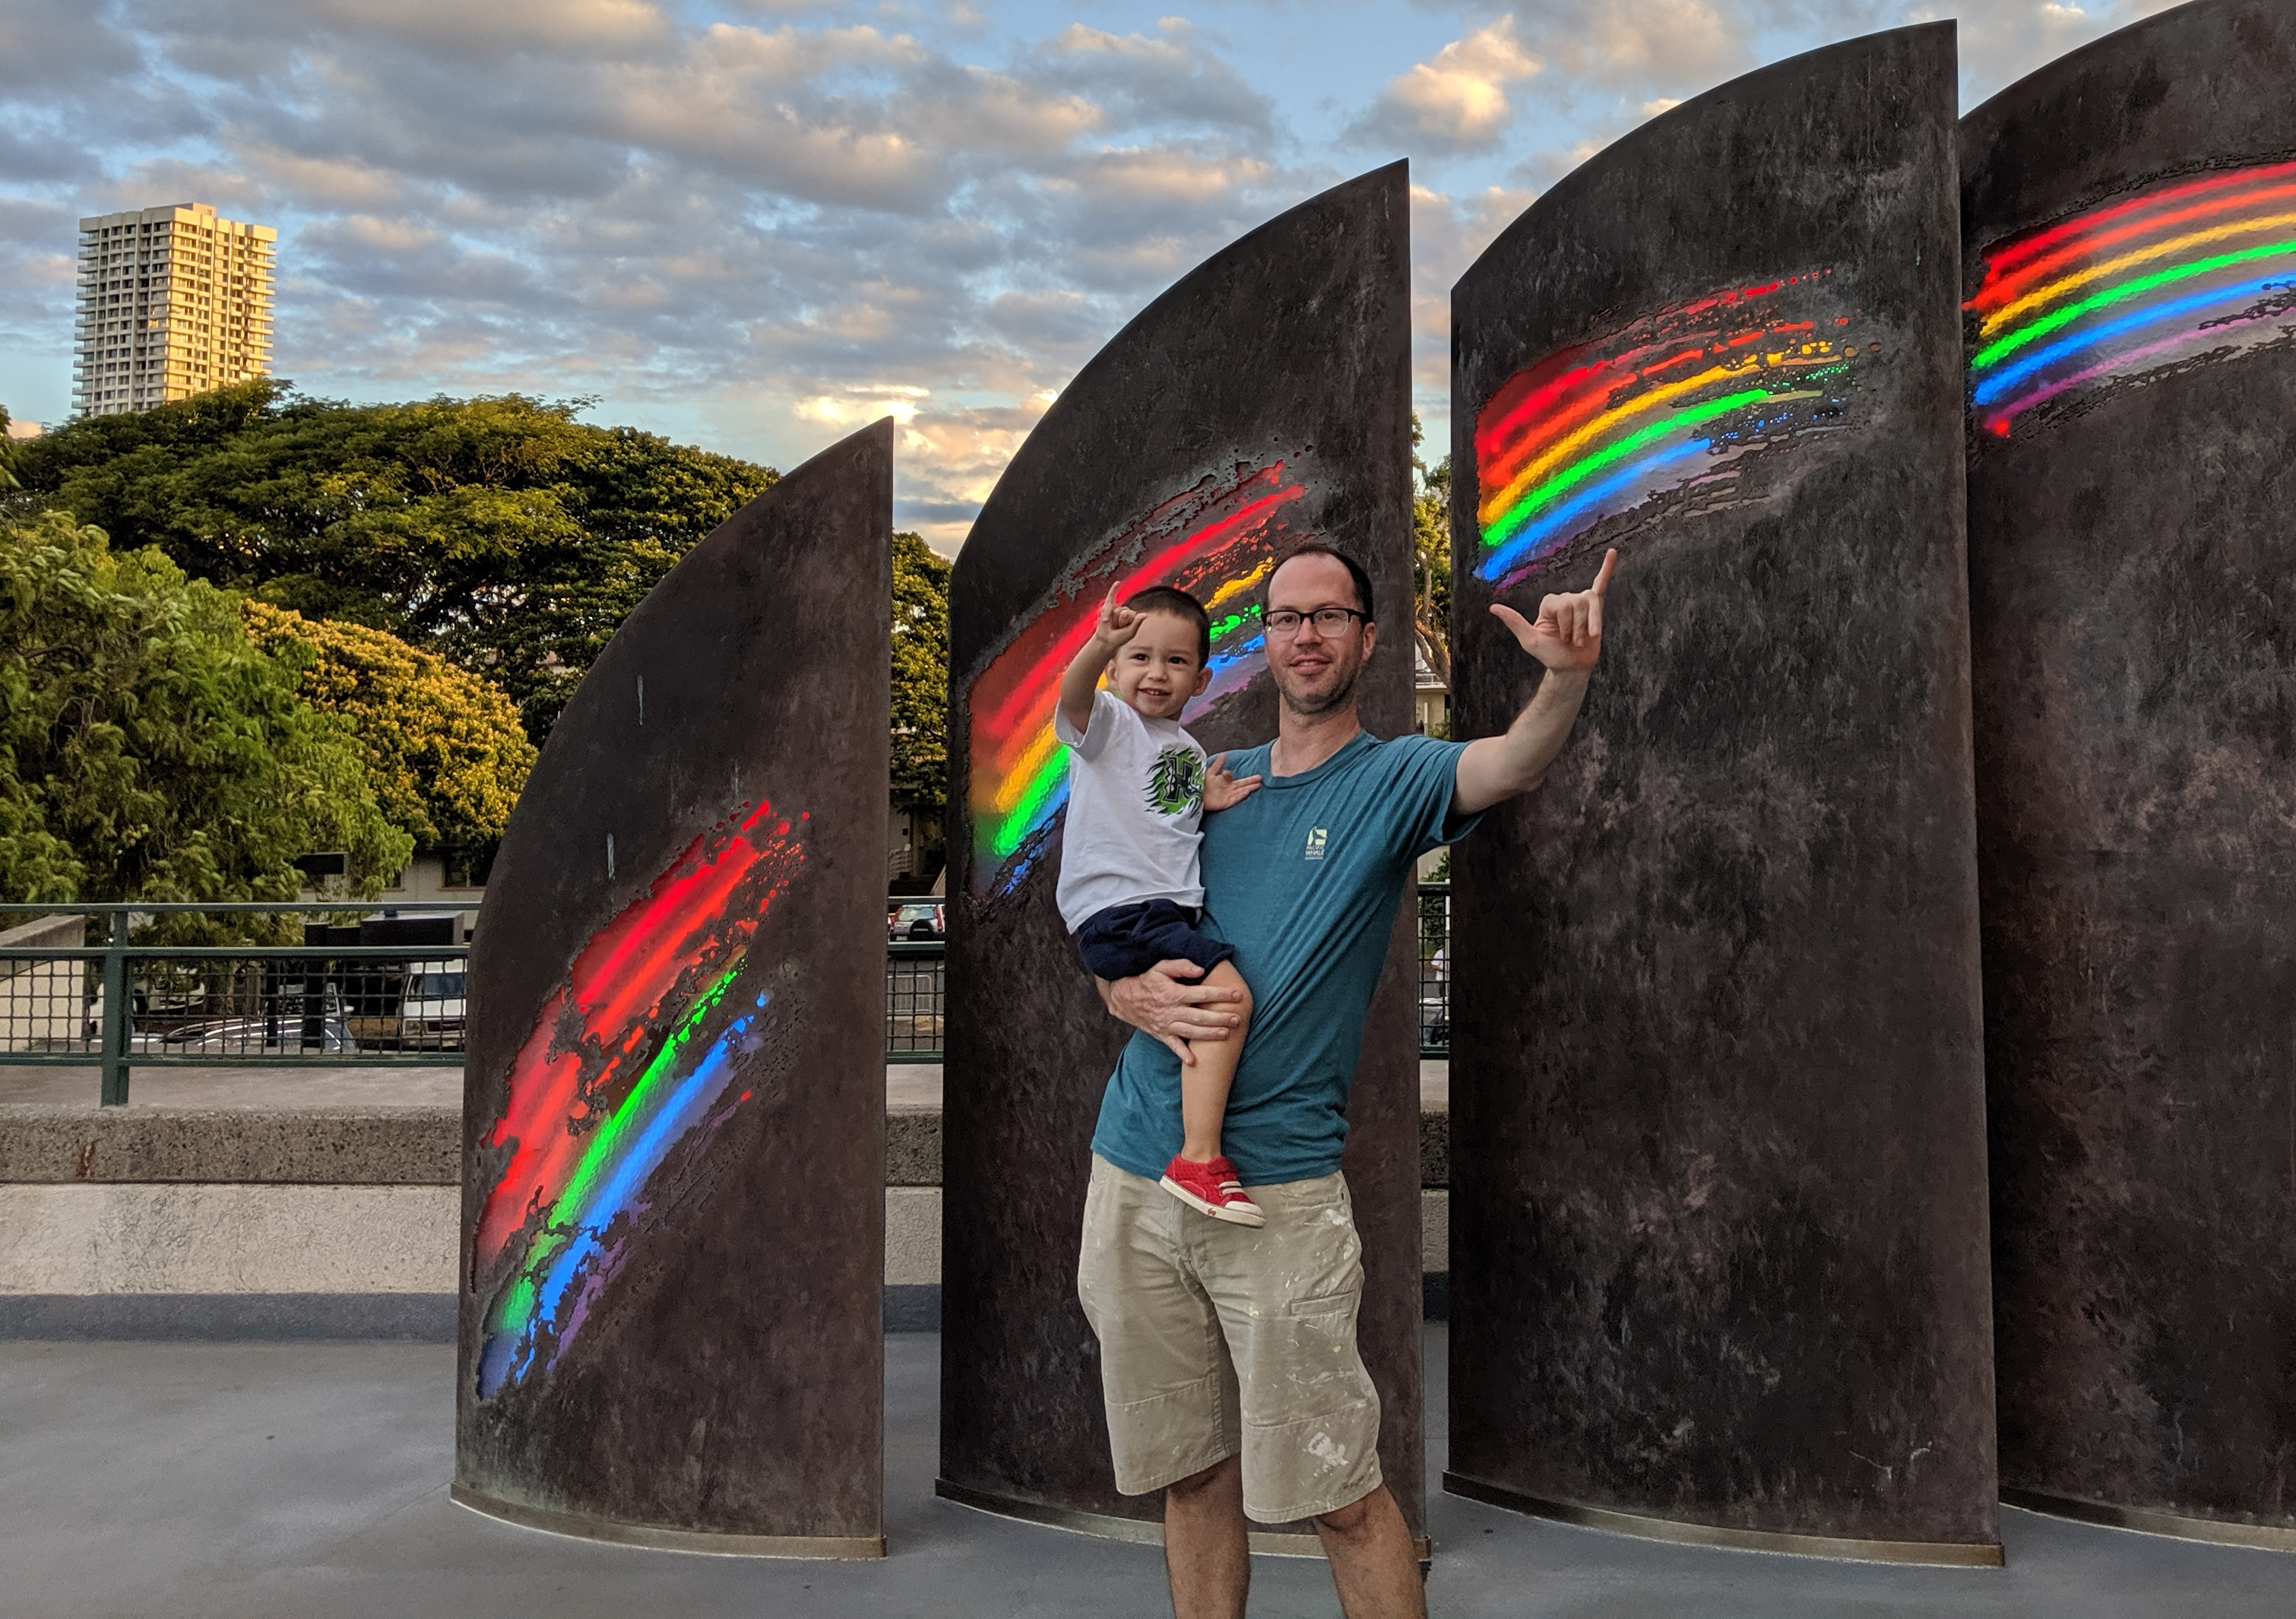
\includegraphics[width=0.75\linewidth]{../Figures/Fergusons} \end{center}

\end{block}

\end{frame}

\begin{frame}{The spread of zebra mussels}
\protect\hypertarget{the-spread-of-zebra-mussels}{}

\note{Hi thanks for coming, today I get to talk to you about counting
zebra mussels. We are going to talk about why something that seems very
simple, going out to a lake and counting ZM's can be improved by using
some ideas from statistics to design these surveys to make sure that we
sample efficiently}

\begin{block}{The Minnesota invasion}

\#\includegraphics{../Figures/MN_animated.gif}

\note{First detected in 1989 in Lake Superior. Mechanisms of spread
natural can be natural dispersal between connected waterways (rivers).
However, human aided dispersal is also an important factor in their
spread. adults can attach to boats, nets, docks, etc. larval zm's can
survive in any bits of water that are not properly drained in boats}

\end{block}

\begin{block}{Impacts of the mussel invasion}

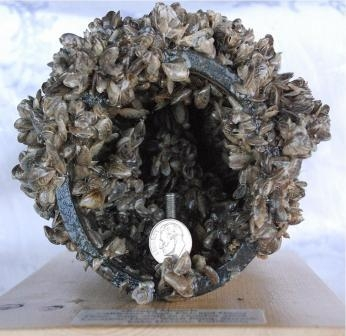
\includegraphics{../Figures/ZebraPipe.jpg}\\
 image: Mussel Prevention Program, San Luis Obispo County

\begin{itemize}
\tightlist
\item
  Changes in water chemistry
\item
  Decreases in plankton densities

  \begin{itemize}
  \tightlist
  \item
    Decreases in native mussel populations
  \item
    Changes in water clarity
  \item
    Increases in plant cover
  \end{itemize}
\item
  Economic impacts on power industry
\end{itemize}

\note{t has been documented that zms can alter their environment by
increasing ammonium and nitrate There have been a number of documented
changes in water chemistry, water clarity Decreases in plankton
production mean less food for fish

economic impacts The photo on the right The zms can occur at extremely
high densities growing over each other in like cancerous cells. They can
reag such high densities can clog intake pipes for industrial
applications. Congressional researchers estimated that an infestation of
zebra mussel in the Great Lakes cost the power industry alone \$3.1
billion in the 1993-1999 period}

\end{block}

\begin{block}{Managing the invasion}

At \textbf{high} densities management options are limited

However, at \textbf{low} densities there are management options
depending on:

\begin{itemize}
\tightlist
\item
  the spatial distribution of the population
\item
  the rate of increase of the population
\end{itemize}

\begin{figure}

{\centering 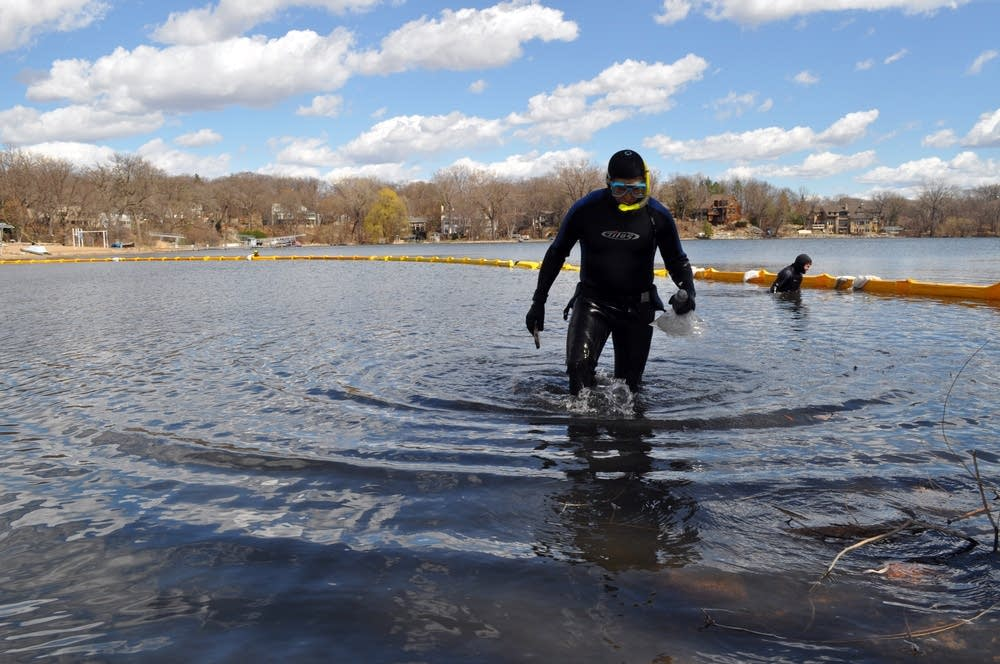
\includegraphics[width=400px]{../Figures/DiversChristmas} 

}

\caption{image:https://www.mprnews.org/story/2015/10/23/zebra-mussels}\label{fig:unnamed-chunk-2}
\end{figure}

\end{block}

\end{frame}

\begin{frame}{Surveying mussels: Year 1}
\protect\hypertarget{surveying-mussels-year-1}{}

\begin{block}{Year 1 field crew}

\begin{figure}

{\centering \includegraphics[width=600px]{../Figures/FieldCrew} 

}

\caption{Photo credit: Naomi Blinick}\label{fig:unnamed-chunk-3}
\end{figure}

\end{block}

\begin{block}{Why shouldn't we just go out and start counting?}

\begin{figure}

{\centering 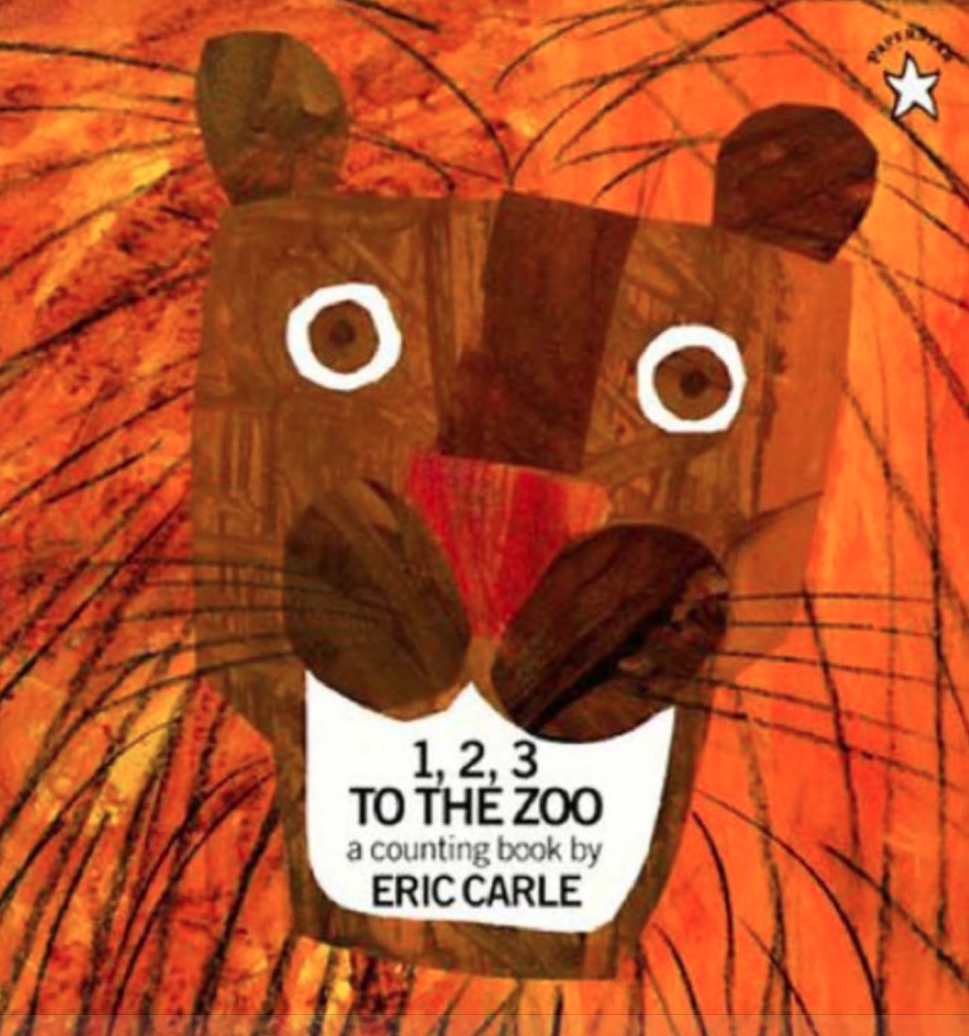
\includegraphics[width=400px]{../Figures/123_zoo} 

}

\caption{image: books.google.com}\label{fig:unnamed-chunk-4}
\end{figure}

\end{block}

\begin{block}{Existing survey designs}

~\\
image: Naomi Blinick

\begin{itemize}
\tightlist
\item
  Discovery in low densities (\textbf{timed searches})
\item
  High-densities (\textbf{quadrat surveys})
\end{itemize}

\textbf{But what about estimating density at low to moderate densities?}

\note{There are a number of different ways that biologists count
critters in the field. For our purposes we are interested in surveying
lakes with low enough densities that simply jumping in the lake and
looking that the bottom will not likely yield useful data. Therefore we
are designing our study around transects, which allow our scuba-diving
field scientists to spend enough time underwater to obtain estimates. We
will have a demonstration at the end of this talk describing this
process in more detail, but for now you can think of it as a line where
the scientist counts the number of organisms on either side.}

\end{block}

\begin{block}{Transect sampling is one approach to cover area quickly}

\begin{center}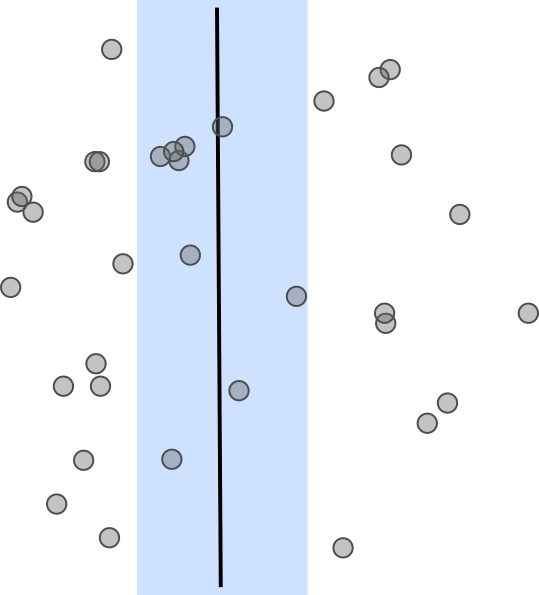
\includegraphics[width=0.4\linewidth]{../Figures/TransectSampling} \end{center}

\end{block}

\begin{block}{Distance sampling is one approach to cover area quickly
\emph{and account for imperfect detection}}

\begin{center}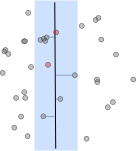
\includegraphics[width=0.4\linewidth]{../Figures/DistanceSampling} \end{center}

\end{block}

\begin{block}{Extra information yields detection estimates}

 Leca, J., N. Gunst, A. Rompis, G. Soma, I. G. A. Arta Putra, and I. N.
Wandia (2013) \emph{Population Density and Abundance of Ebony Leaf
Monkeys (Trachypithecus auratus) in West Bali National Park, Indonesia},
Primate Conservation 26(1), 133-144.

\end{block}

\begin{block}{Important assumptions in conventional distance sampling}

\begin{itemize}
\tightlist
\item
  Density away from transect line is homogenous
\item
  Detection on the transect line is \emph{perfect}
\item
  Animals do not move before detection
\item
  Measurements are exact
\end{itemize}

\end{block}

\begin{block}{First lake: Lake Sylvia}

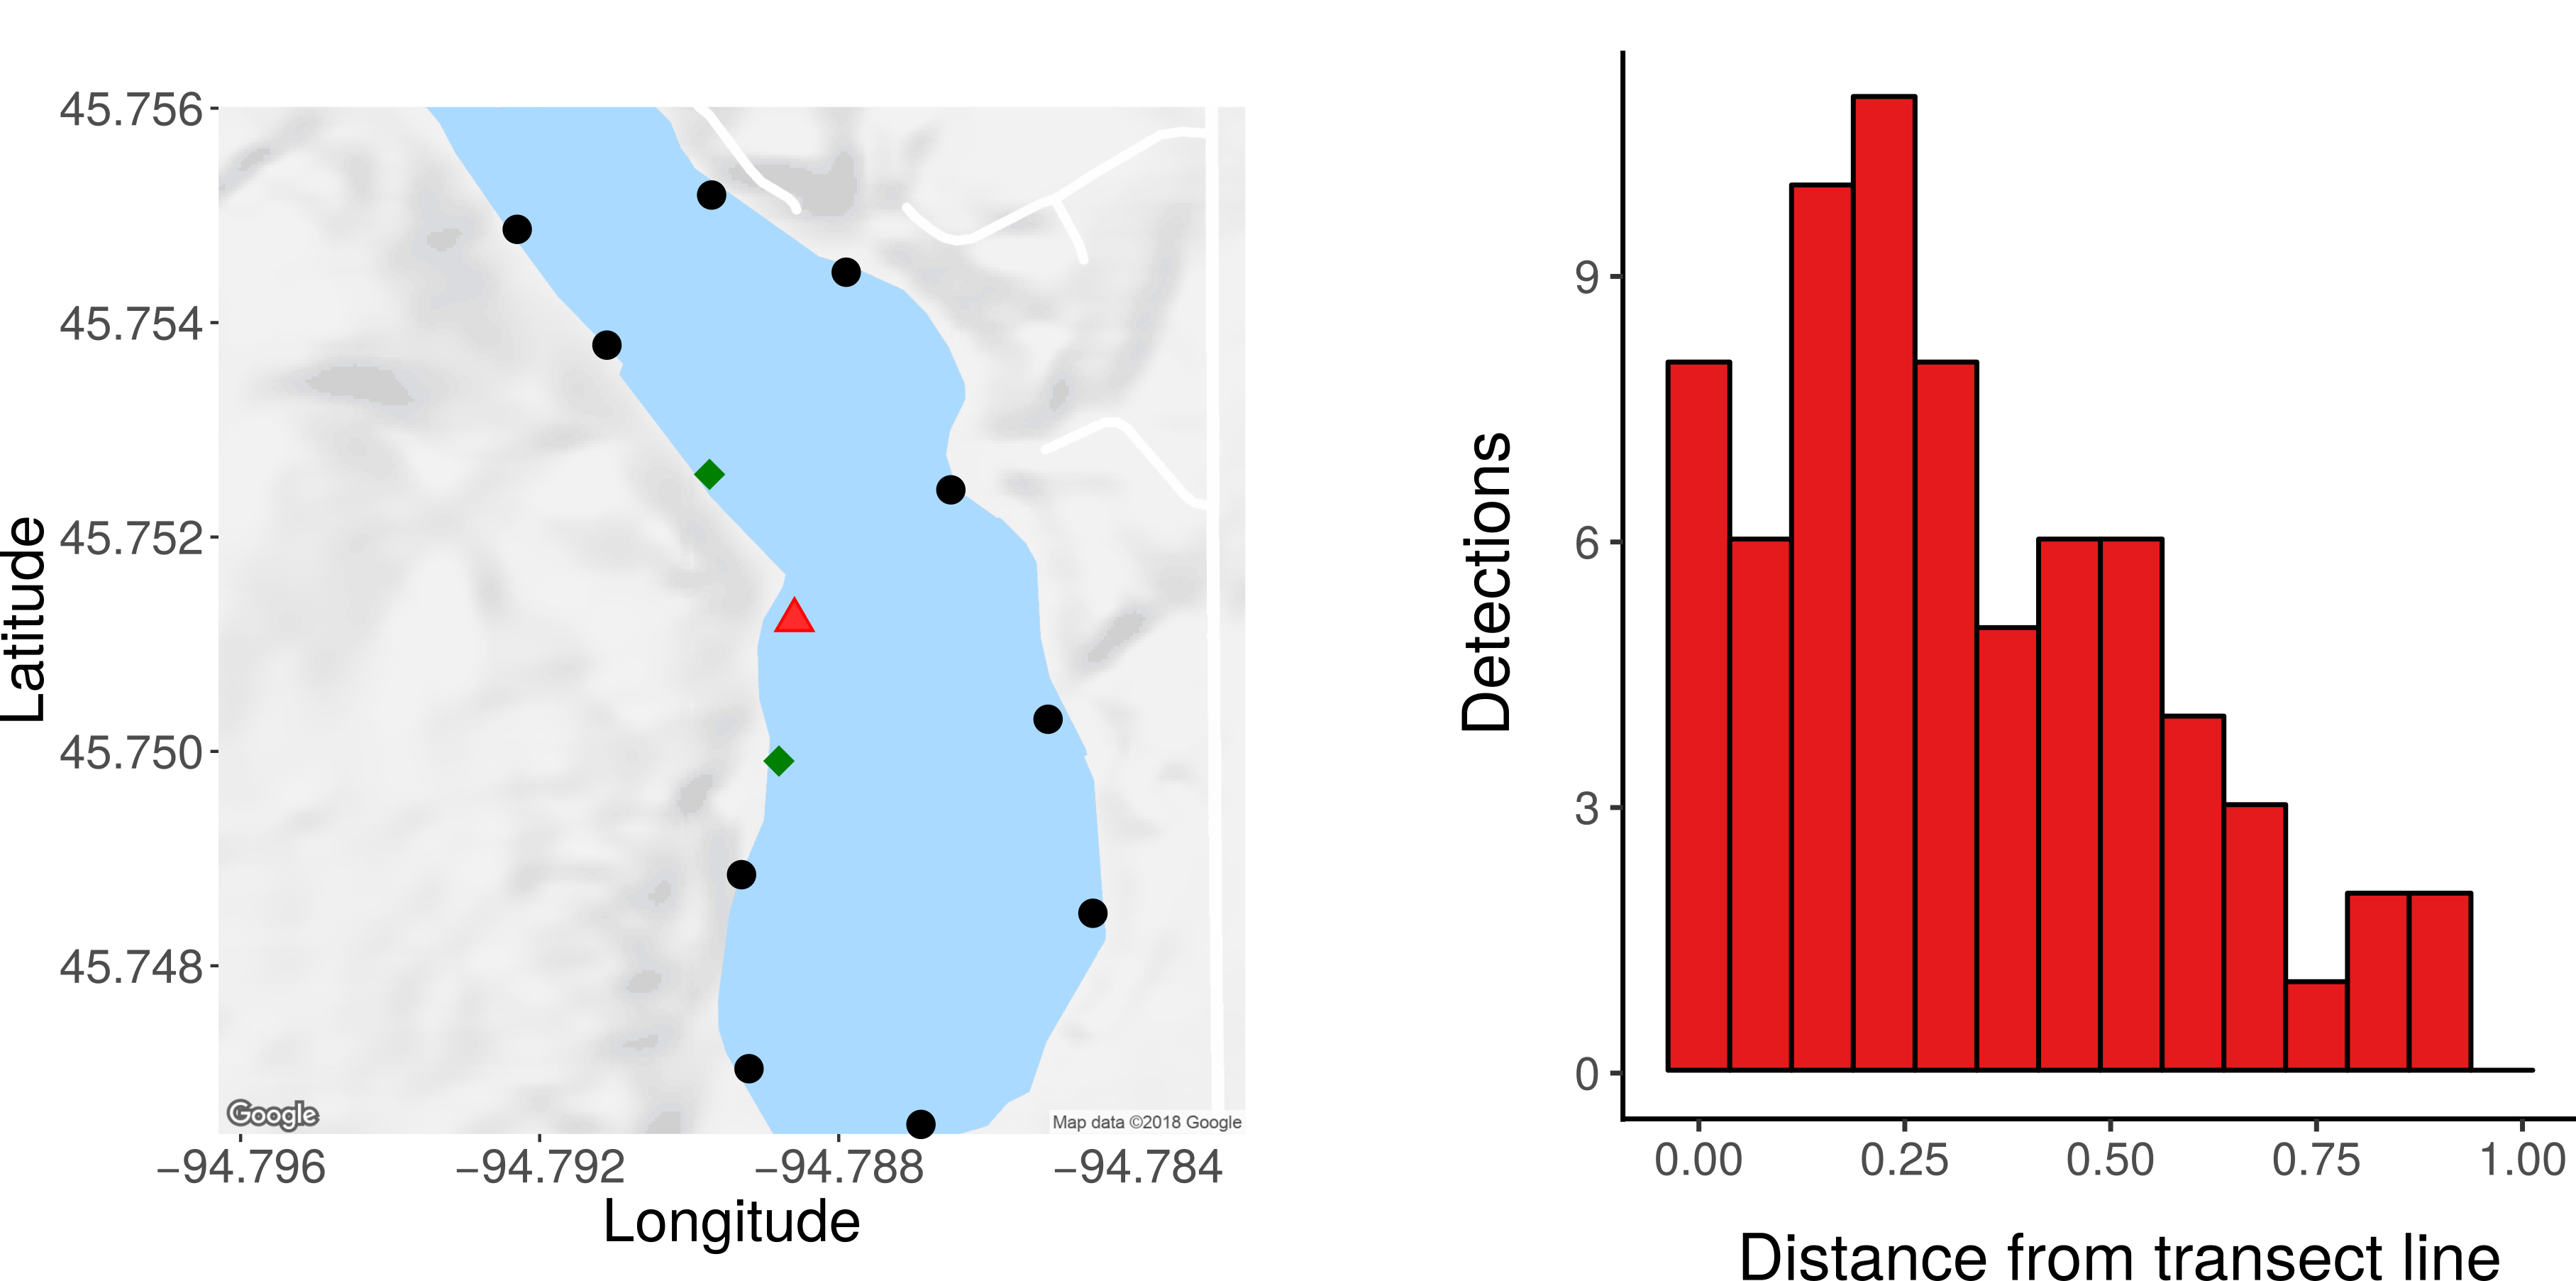
\includegraphics[width=0.9\linewidth]{../Figures/SylviaSummary}

Note the hump shape, are we detecting everything on the transect line?

\end{block}

\begin{block}{We needed to add a second observer!}

\begin{itemize}
\tightlist
\item
  Adds a mark-recap component to the distance survey.

  \begin{itemize}
  \tightlist
  \item
    First diver counts, followed by second diver
  \end{itemize}
\item
  Determining which mussels are detected by one or both observers allows
  us to estimate density on the transect line.
\end{itemize}

\end{block}

\begin{block}{Second lake: Lake Burgan}

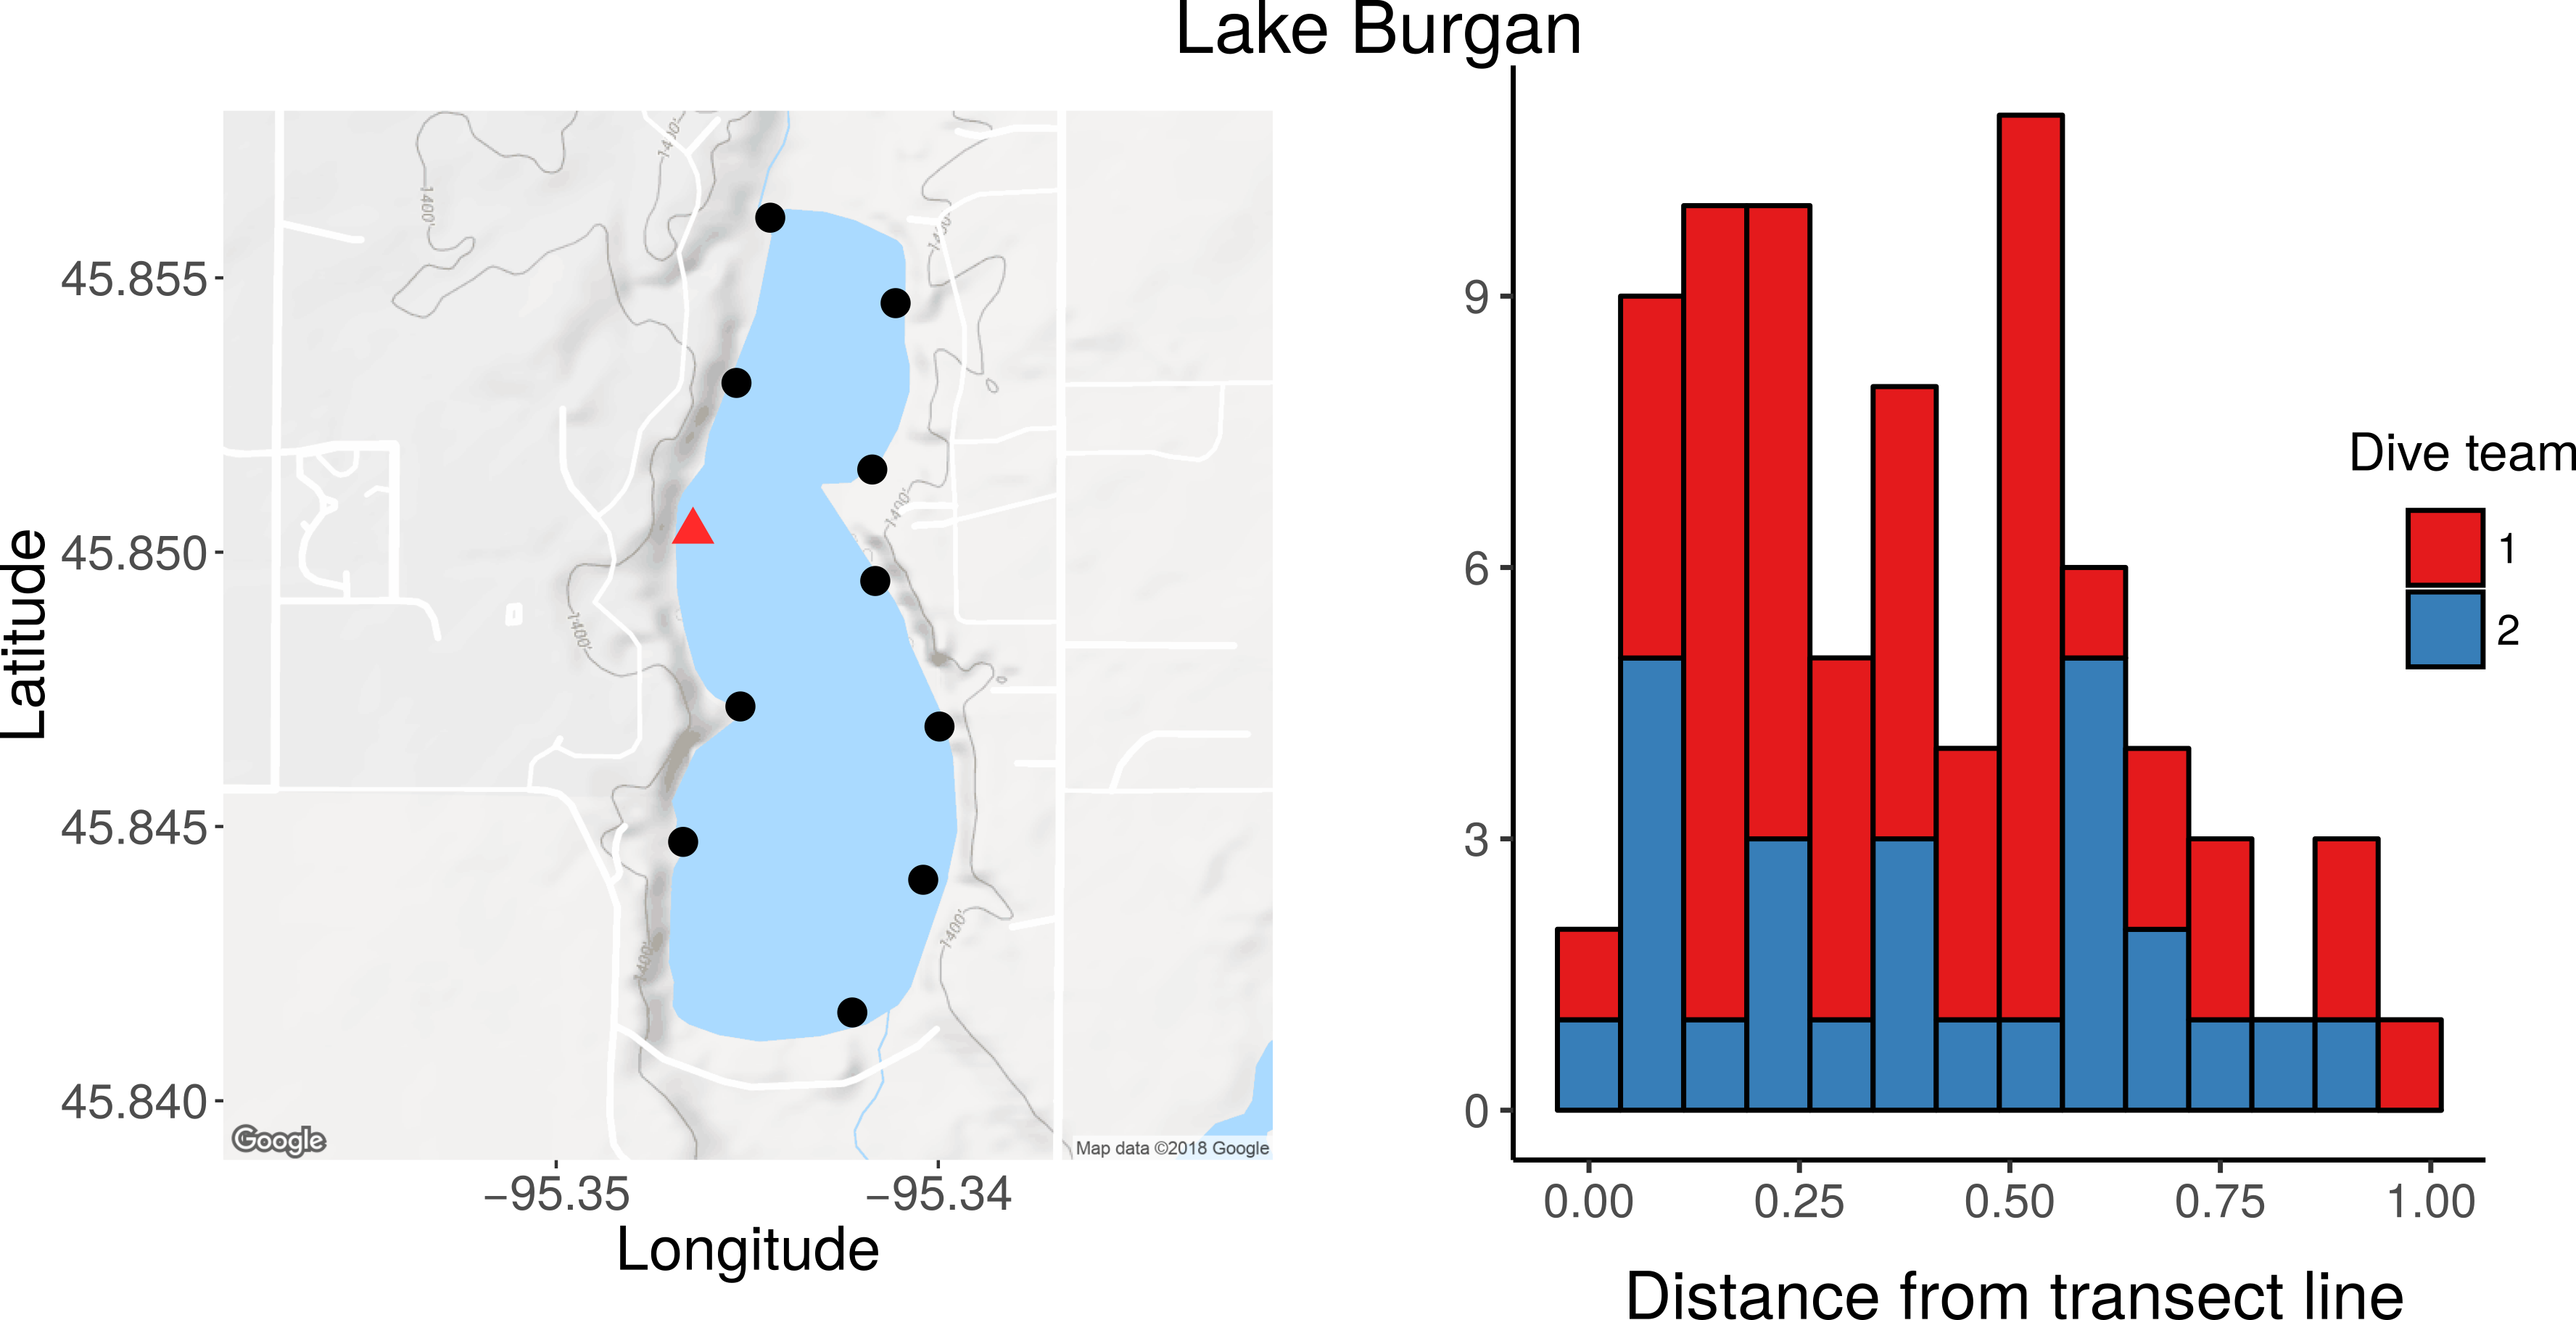
\includegraphics[width=0.9\linewidth]{../Figures/BurganSummary}

\end{block}

\begin{block}{We can now estimate detection probabilities}

\begin{figure}

{\centering 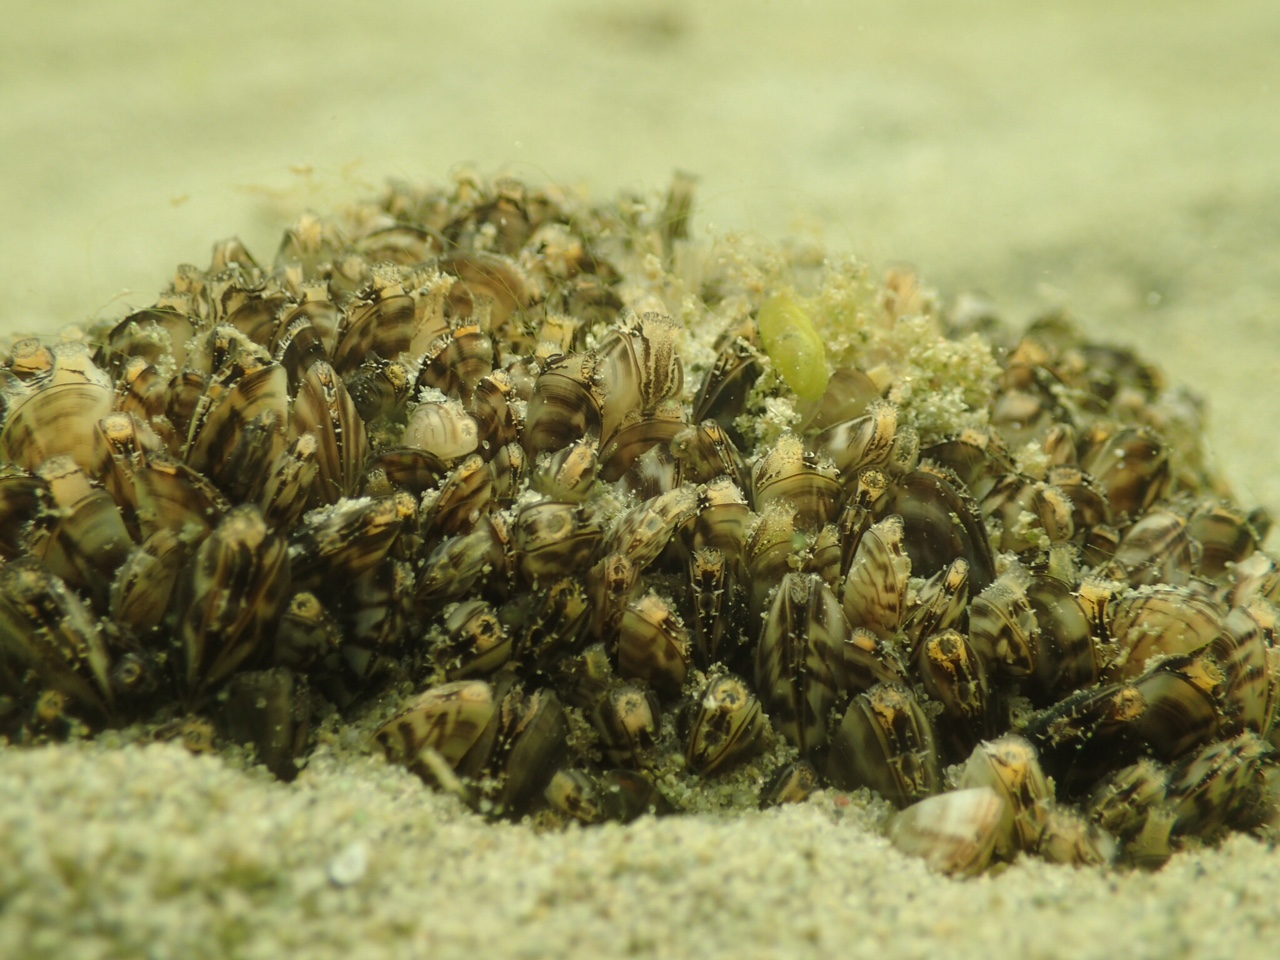
\includegraphics[width=0.7\linewidth]{../Figures/IMG_2558} 

}

\caption{Image credit: Naomi Blinick}\label{fig:unnamed-chunk-9}
\end{figure}

Estimated density without detection \(0.08\) mussels/m\(^2\).

Estimated density without detection \(0.24\) \((0.06)\) mussels/m\(^2\)
.

\end{block}

\begin{block}{Lessons from Year 1}

\begin{itemize}
\tightlist
\item
  Detection on the transect line is far from perfect
\item
  Need to use double-observer surveys

  \begin{itemize}
  \tightlist
  \item
    Significant heterogeneity \emph{between} observers
  \end{itemize}
\item
  Do not need to stratify effort
\item
  Dive surveys are hard
\end{itemize}

\begin{figure}

{\centering 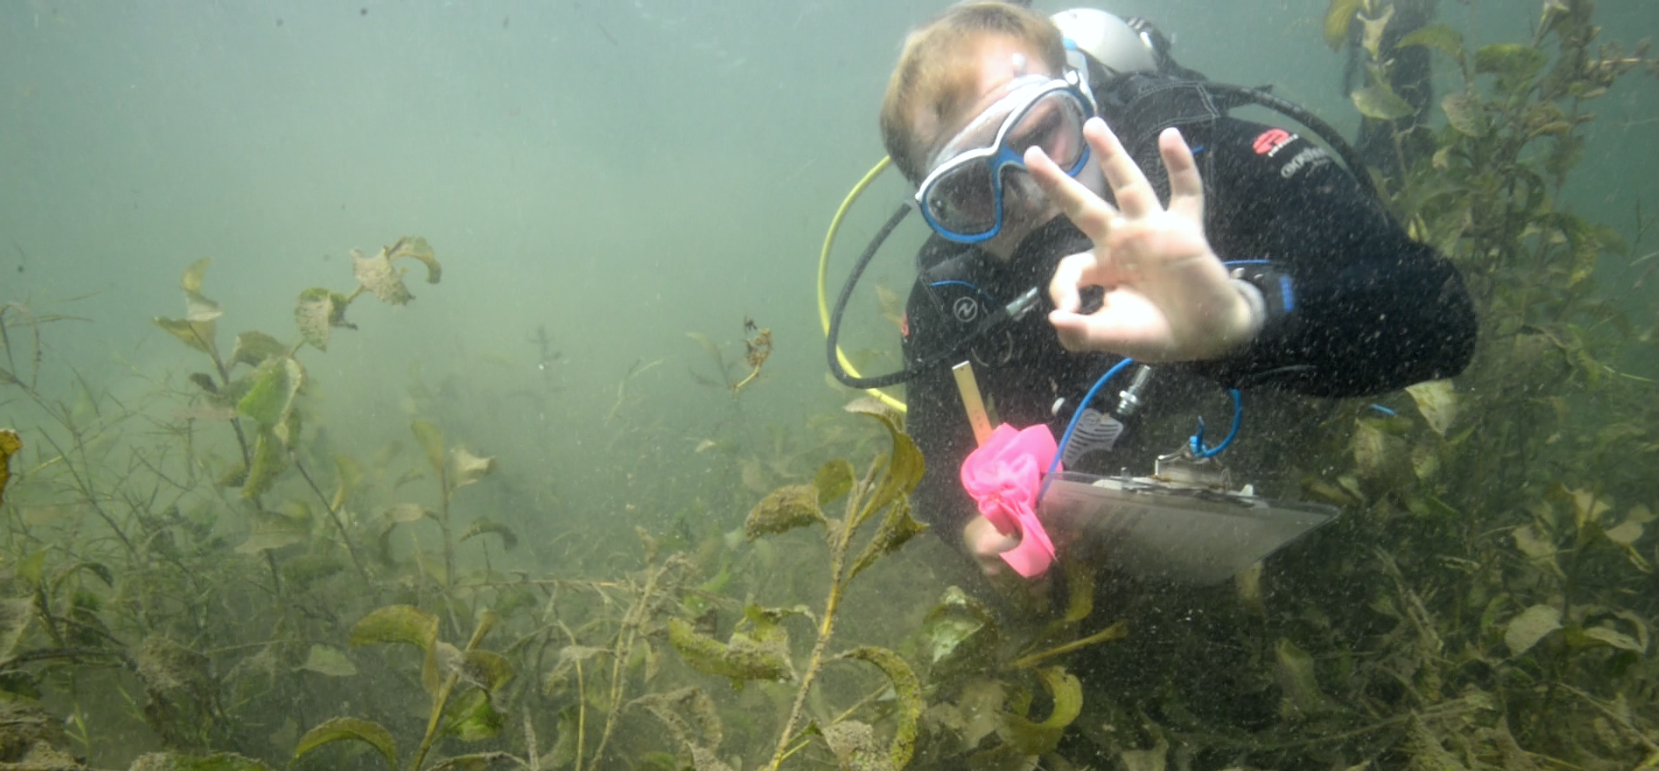
\includegraphics[width=0.6\linewidth]{../Figures/AustenDistance} 

}

\caption{Image credit: Aislyn Keyes}\label{fig:unnamed-chunk-10}
\end{figure}

\end{block}

\end{frame}

\begin{frame}{Surveying mussels: Year 2}
\protect\hypertarget{surveying-mussels-year-2}{}

\begin{block}{Dive team}

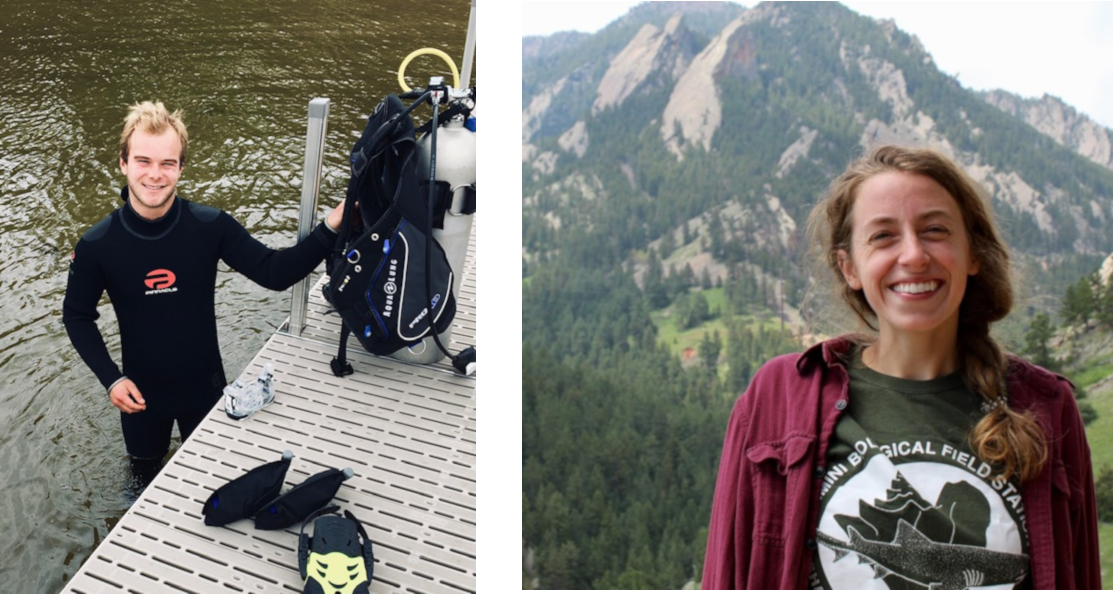
\includegraphics[width=0.9\linewidth]{../Figures/Season2Group}

\end{block}

\begin{block}{But how do distance surveys compare to quadrat surveys?}

Last year we demonstrated that distance surveying is possible, but
(\emph{when}) is it preferable?\\

\begin{figure}

{\centering 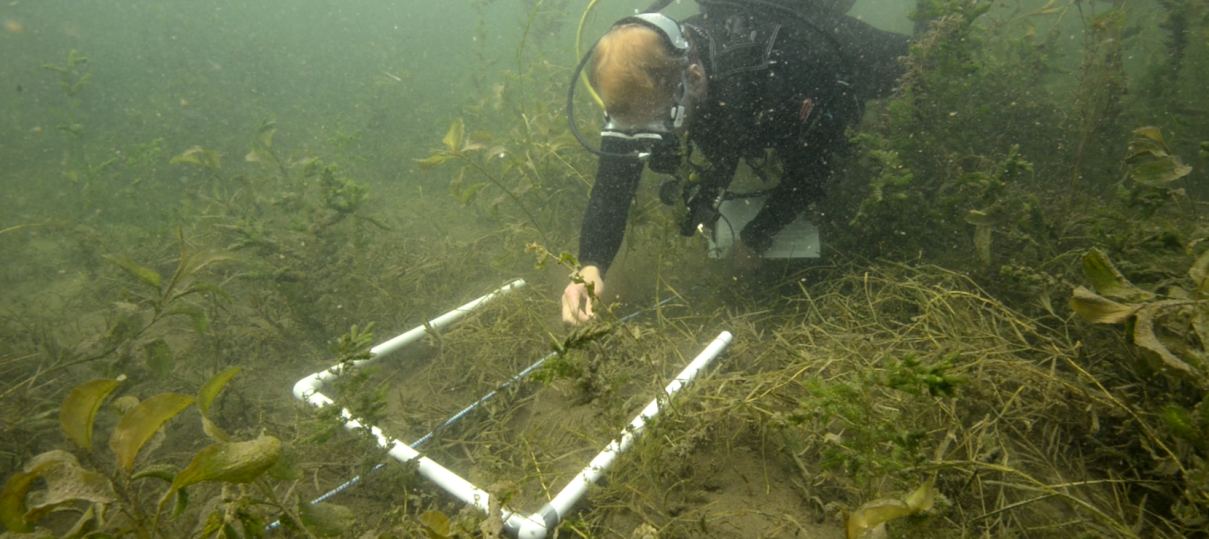
\includegraphics[width=0.6\linewidth]{../Figures/AustenQuad} 

}

\caption{image credit: Jake Ferguson}\label{fig:unnamed-chunk-12}
\end{figure}

\end{block}

\begin{block}{Given a \emph{fixed} amount of time, which method performs
best?}

\begin{center}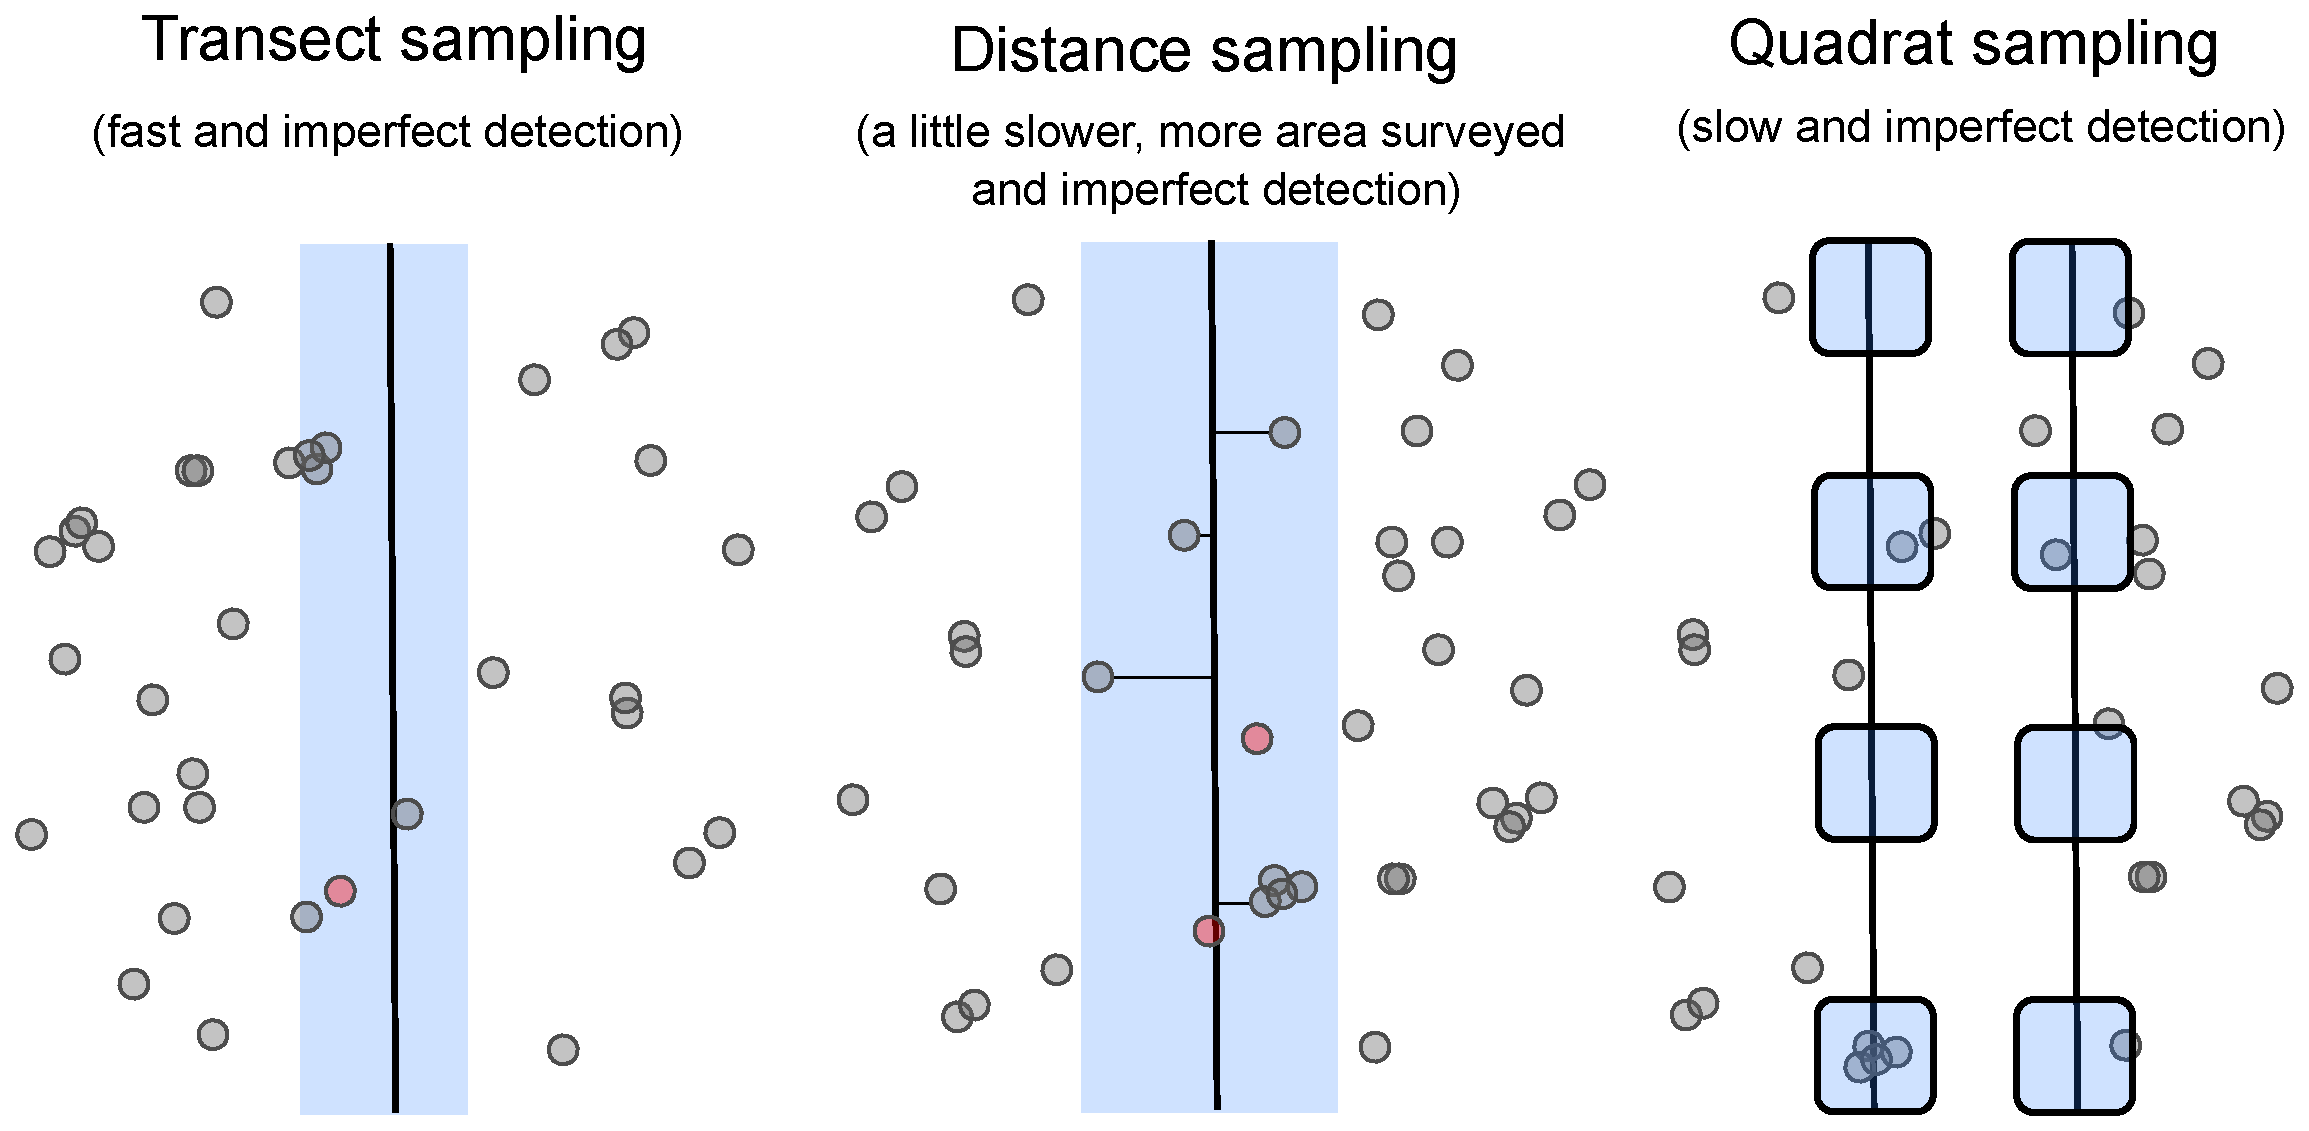
\includegraphics[width=0.6\linewidth]{../Figures/DistanceQuadratSampling} \end{center}

\end{block}

\begin{block}{Two sources of variance: counts and detection}

\begin{center}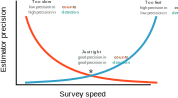
\includegraphics[width=0.7\linewidth]{../Figures/PrecisionTradeoffs} \end{center}

\end{block}

\begin{block}{Compare designs across densities}

\begin{center}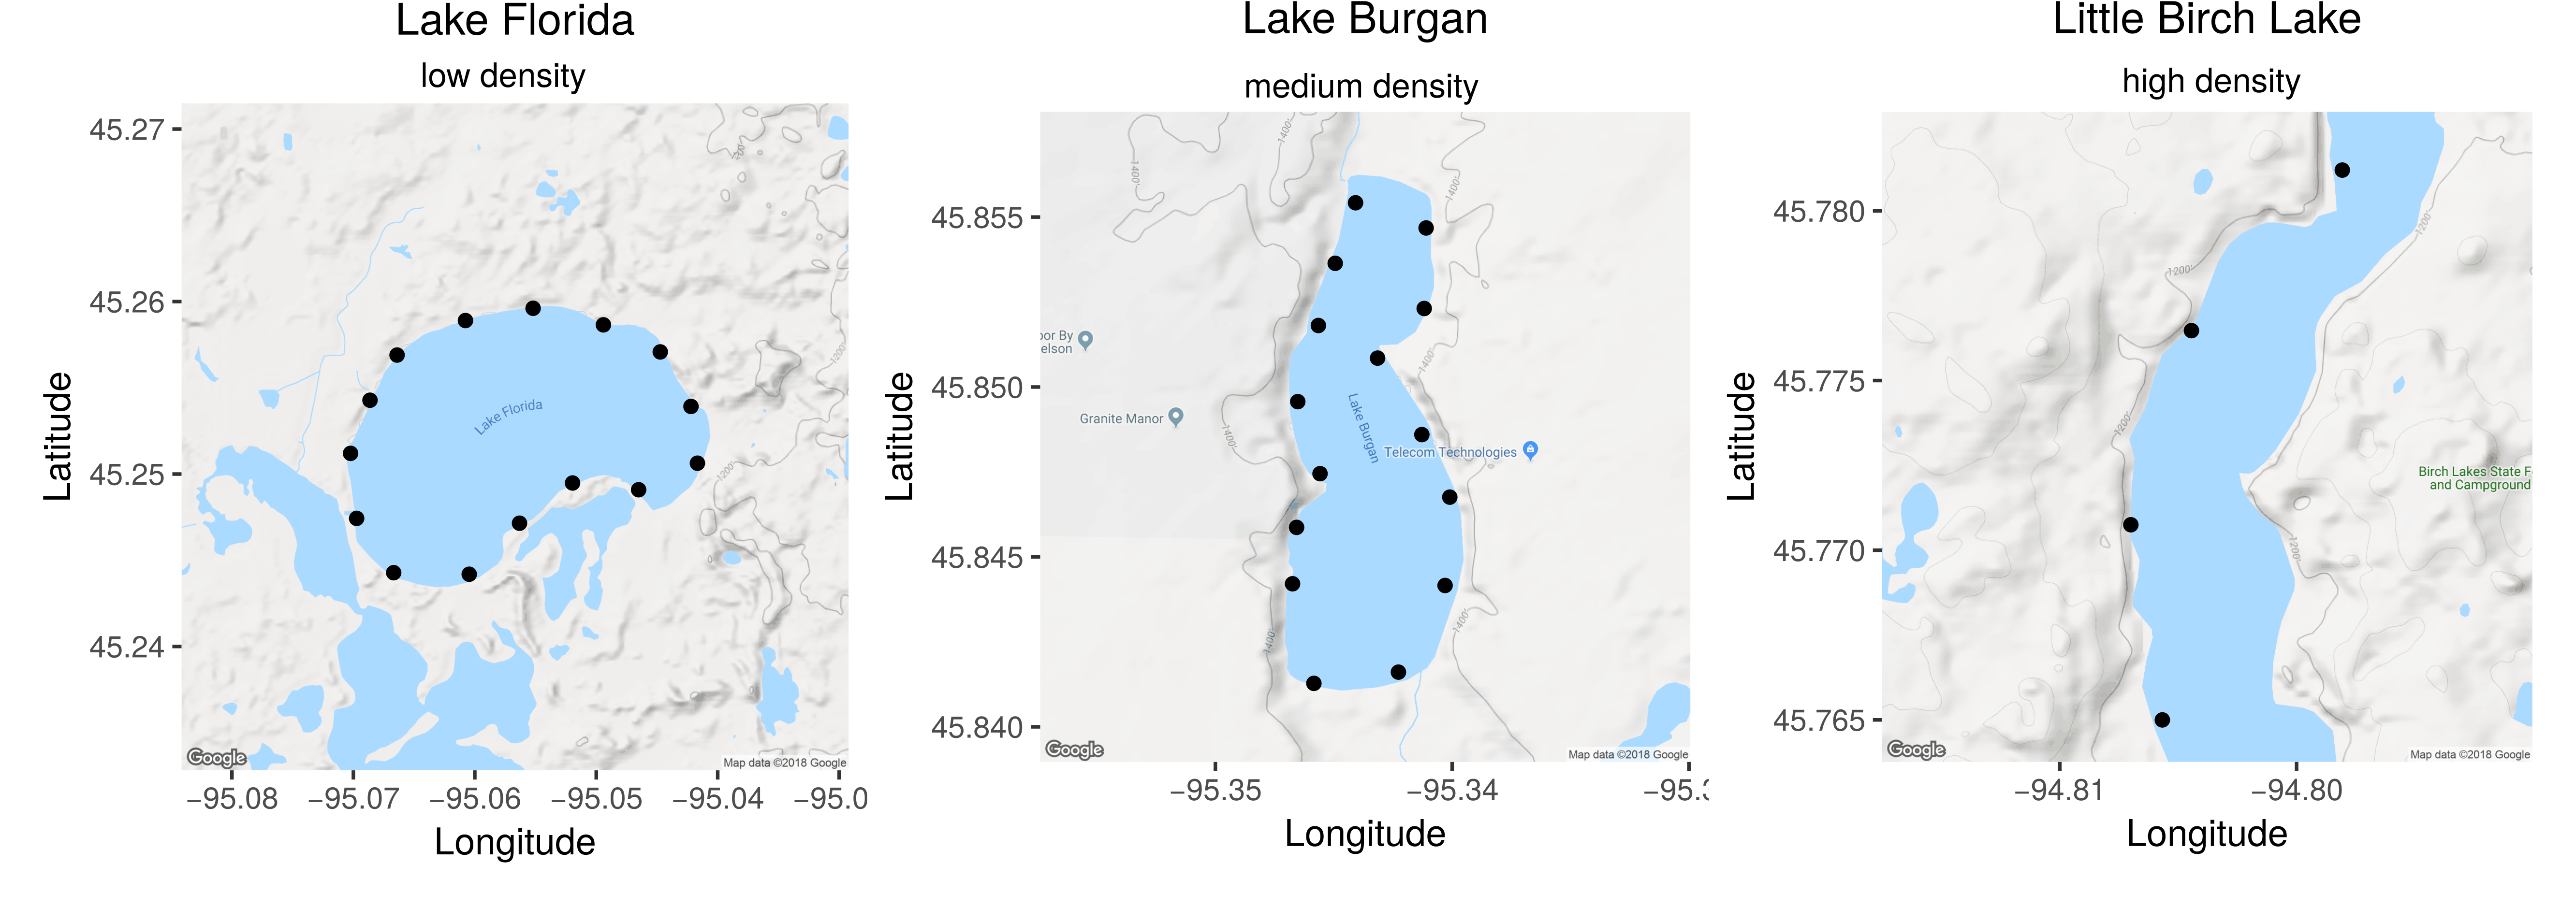
\includegraphics[width=0.95\linewidth]{../Figures/Season2Lakes} \end{center}

\end{block}

\begin{block}{Results}

\begin{center}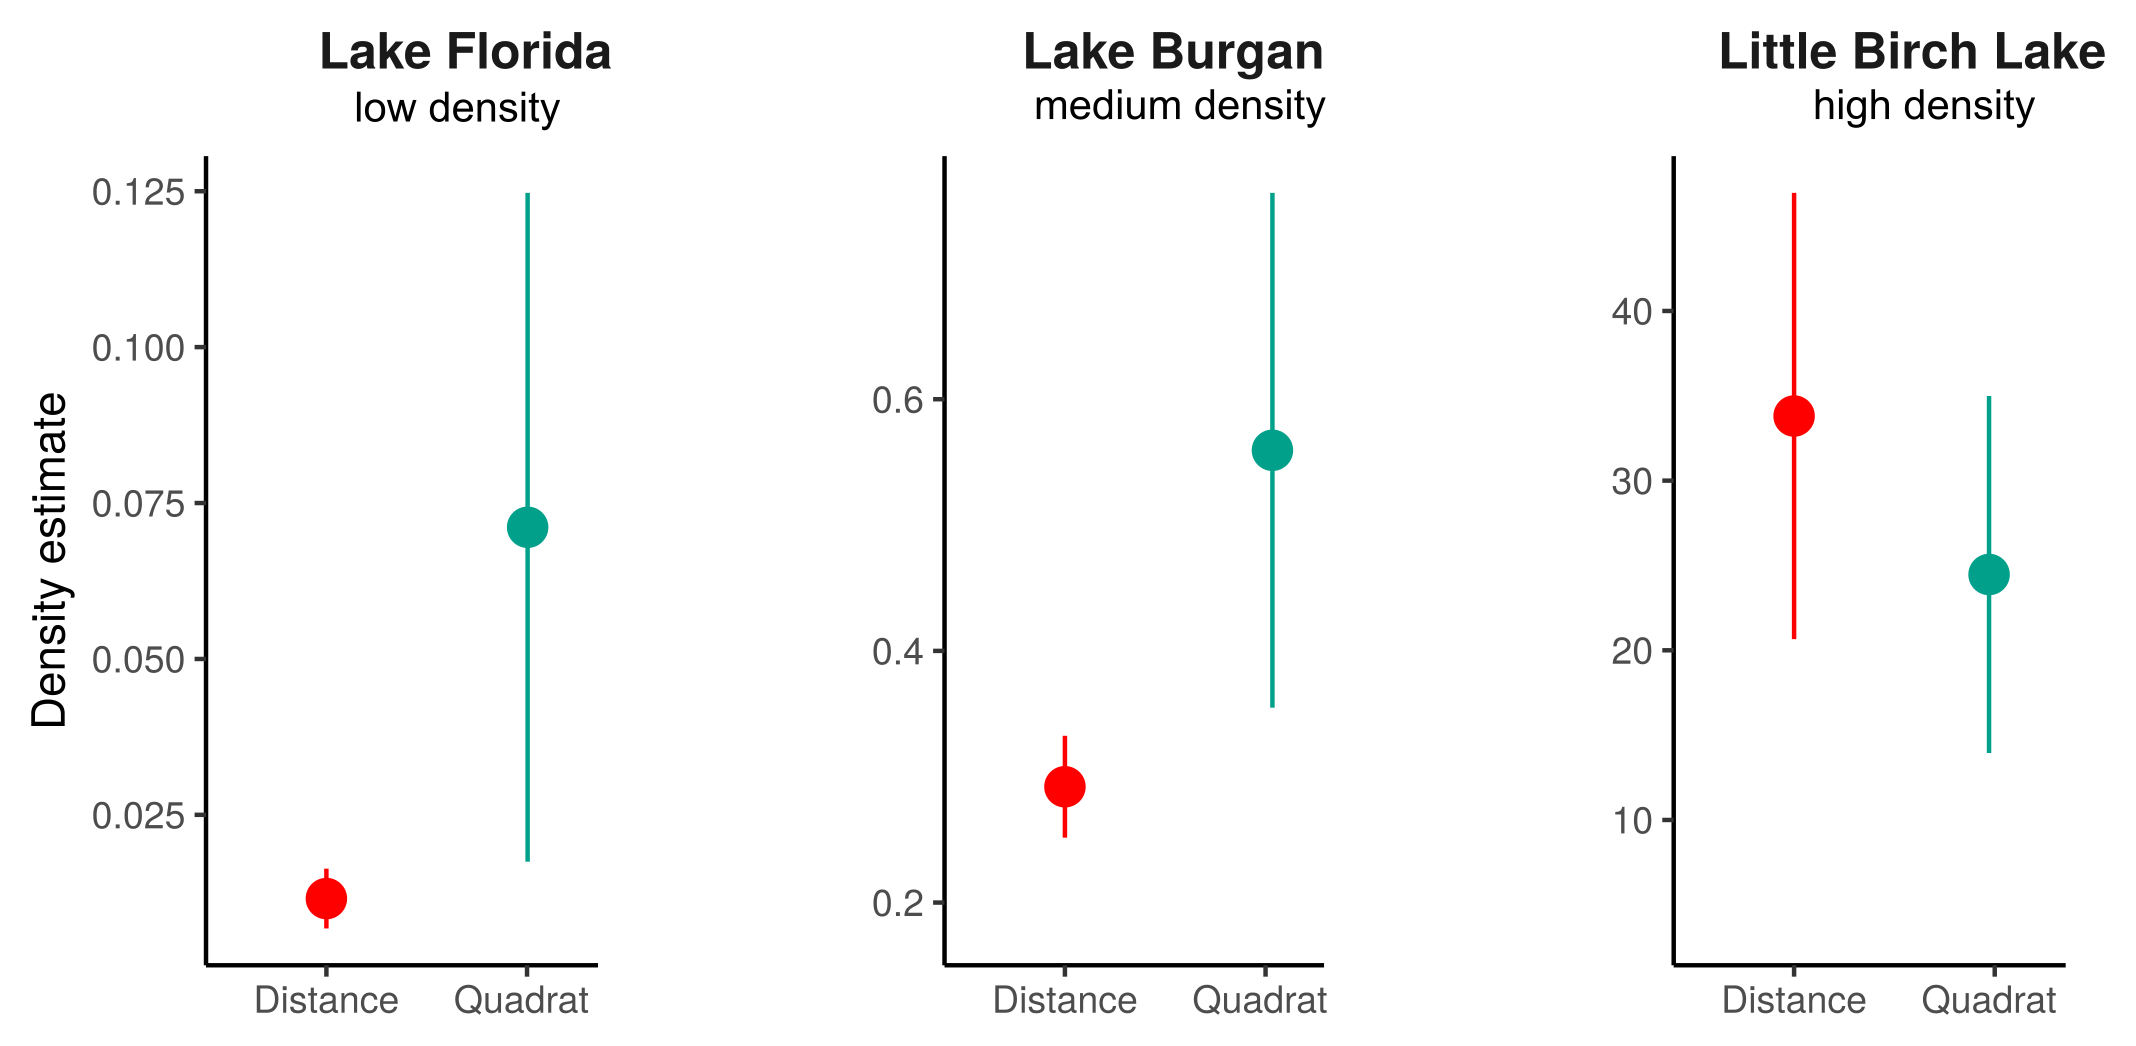
\includegraphics[width=0.9\linewidth]{../Figures/DensityEstimate2} \end{center}

\end{block}

\begin{block}{Lessons from Year 2}

\begin{itemize}
\tightlist
\item
  Distance sampling is preferable at low to moderate densities
\end{itemize}

\begin{figure}

{\centering 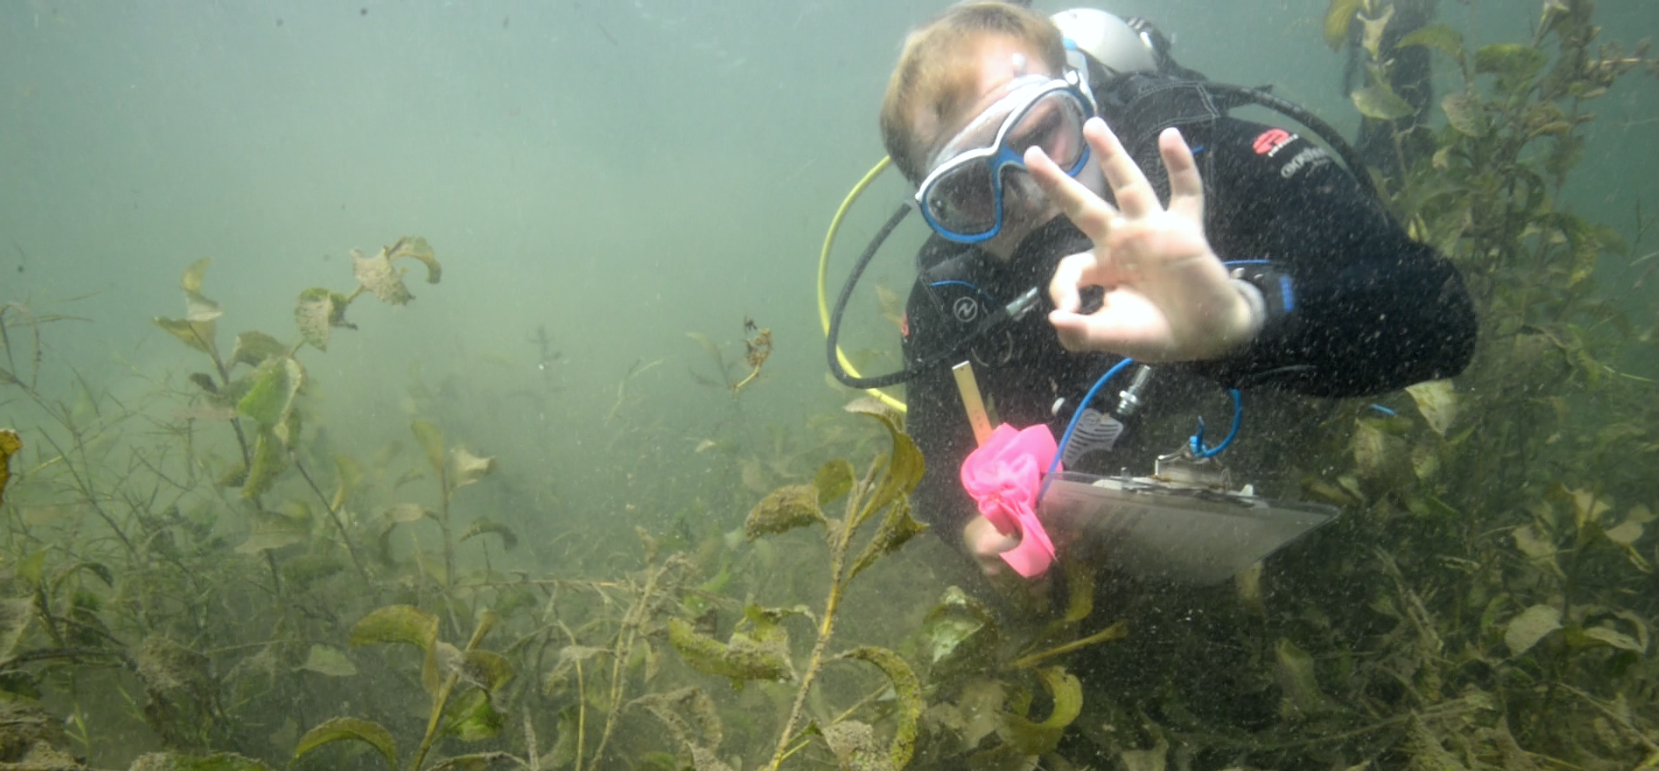
\includegraphics[width=0.7\linewidth]{../Figures/AustenDistance} 

}

\caption{image credit: Aislyn Keyes}\label{fig:unnamed-chunk-17}
\end{figure}

\end{block}

\begin{block}{Other materials}

\begin{center}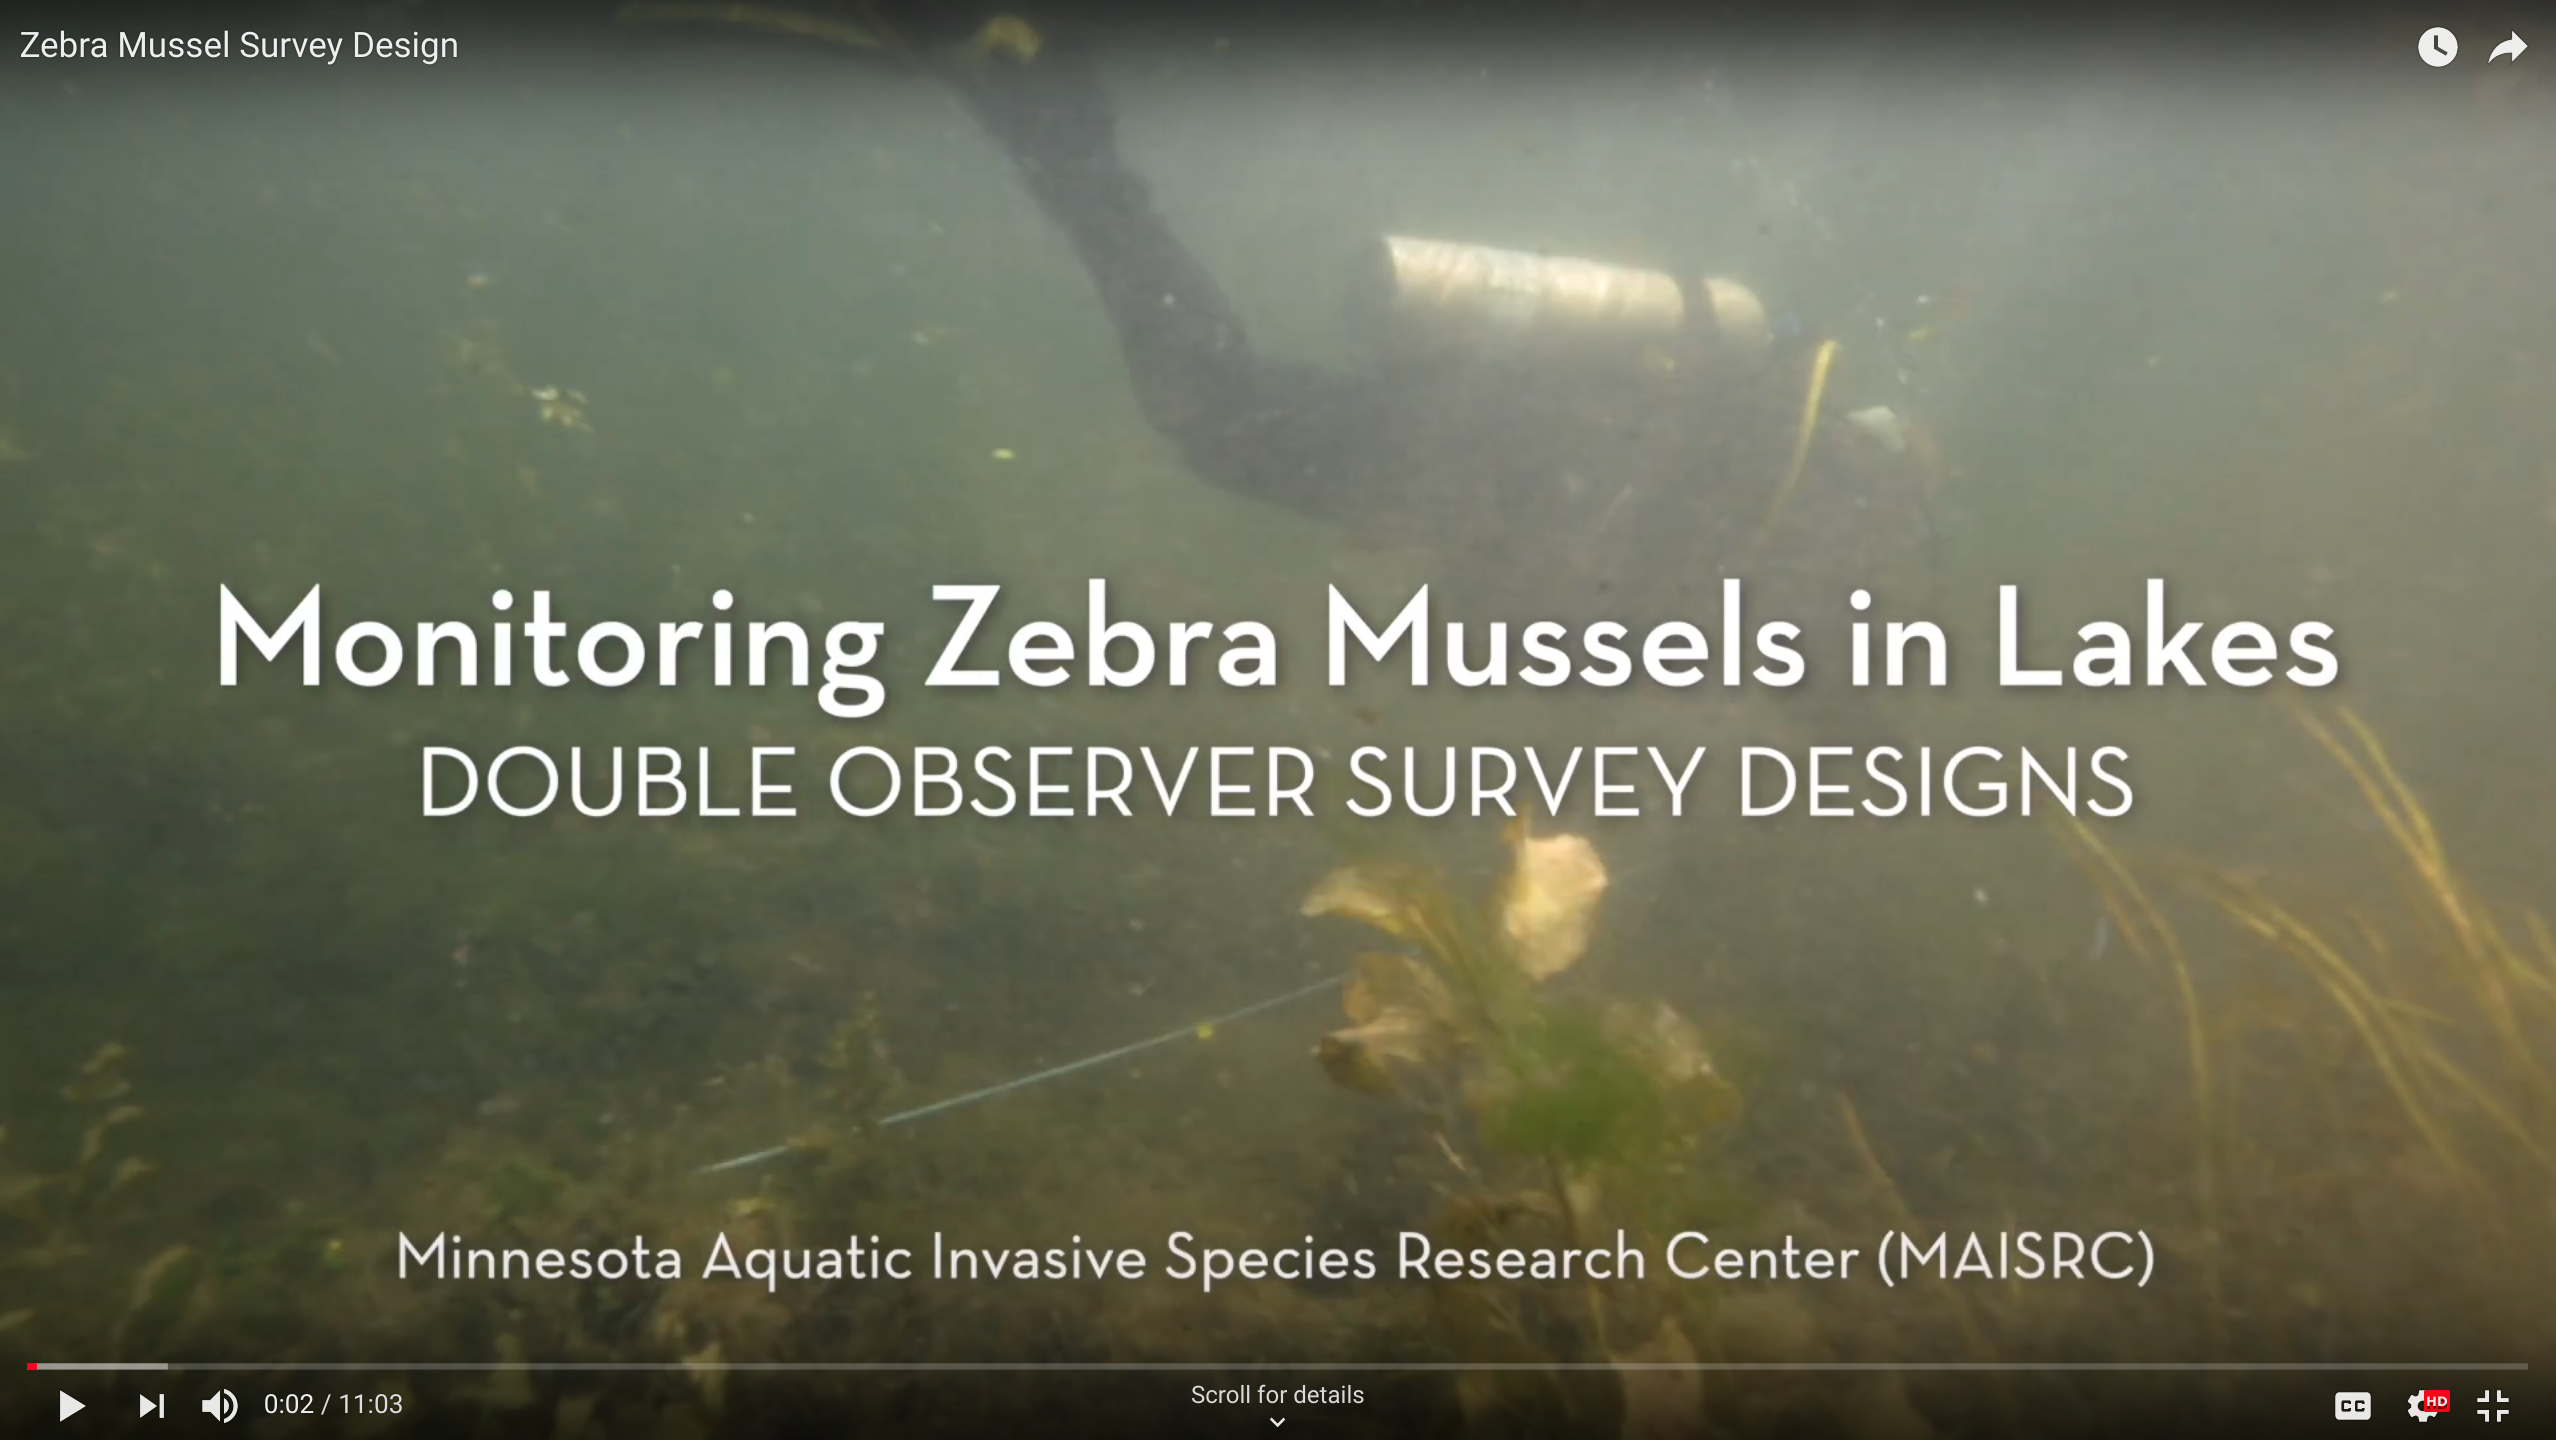
\includegraphics[width=0.7\linewidth]{../Figures/Youtube} \end{center}

Video tutorial: \url{https://youtu.be/E3ui8SVeBC0}

Analysis tutorial: \url{https://zebramusselsurveys.netlify.com/tutorial}

\end{block}

\end{frame}

\begin{frame}{Generalizing these results}
\protect\hypertarget{generalizing-these-results}{}

\begin{block}{Analogy to Optimal Foraging Theory}

\begin{center}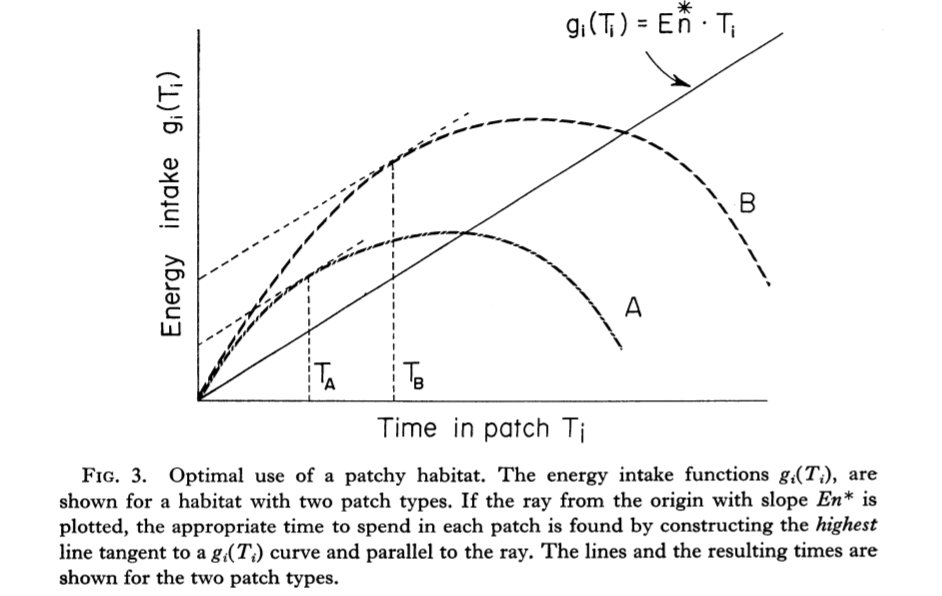
\includegraphics[width=0.8\linewidth]{../Figures/OptForTheory} \end{center}

\end{block}

\begin{block}{Break up the survey into steps, determine the time it
takes to complete each piece}

\begin{center}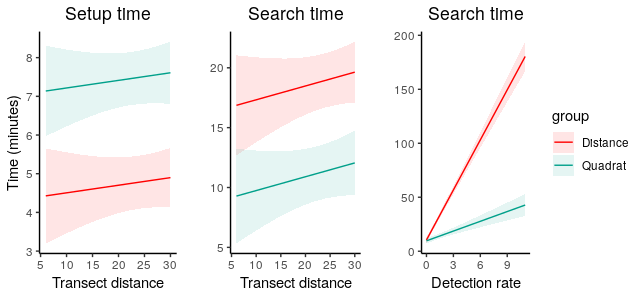
\includegraphics[width=0.8\linewidth]{../Figures/TimeBudgetEstimates} \end{center}

\end{block}

\begin{block}{We can use this to predict the optimal strategy}

\begin{center}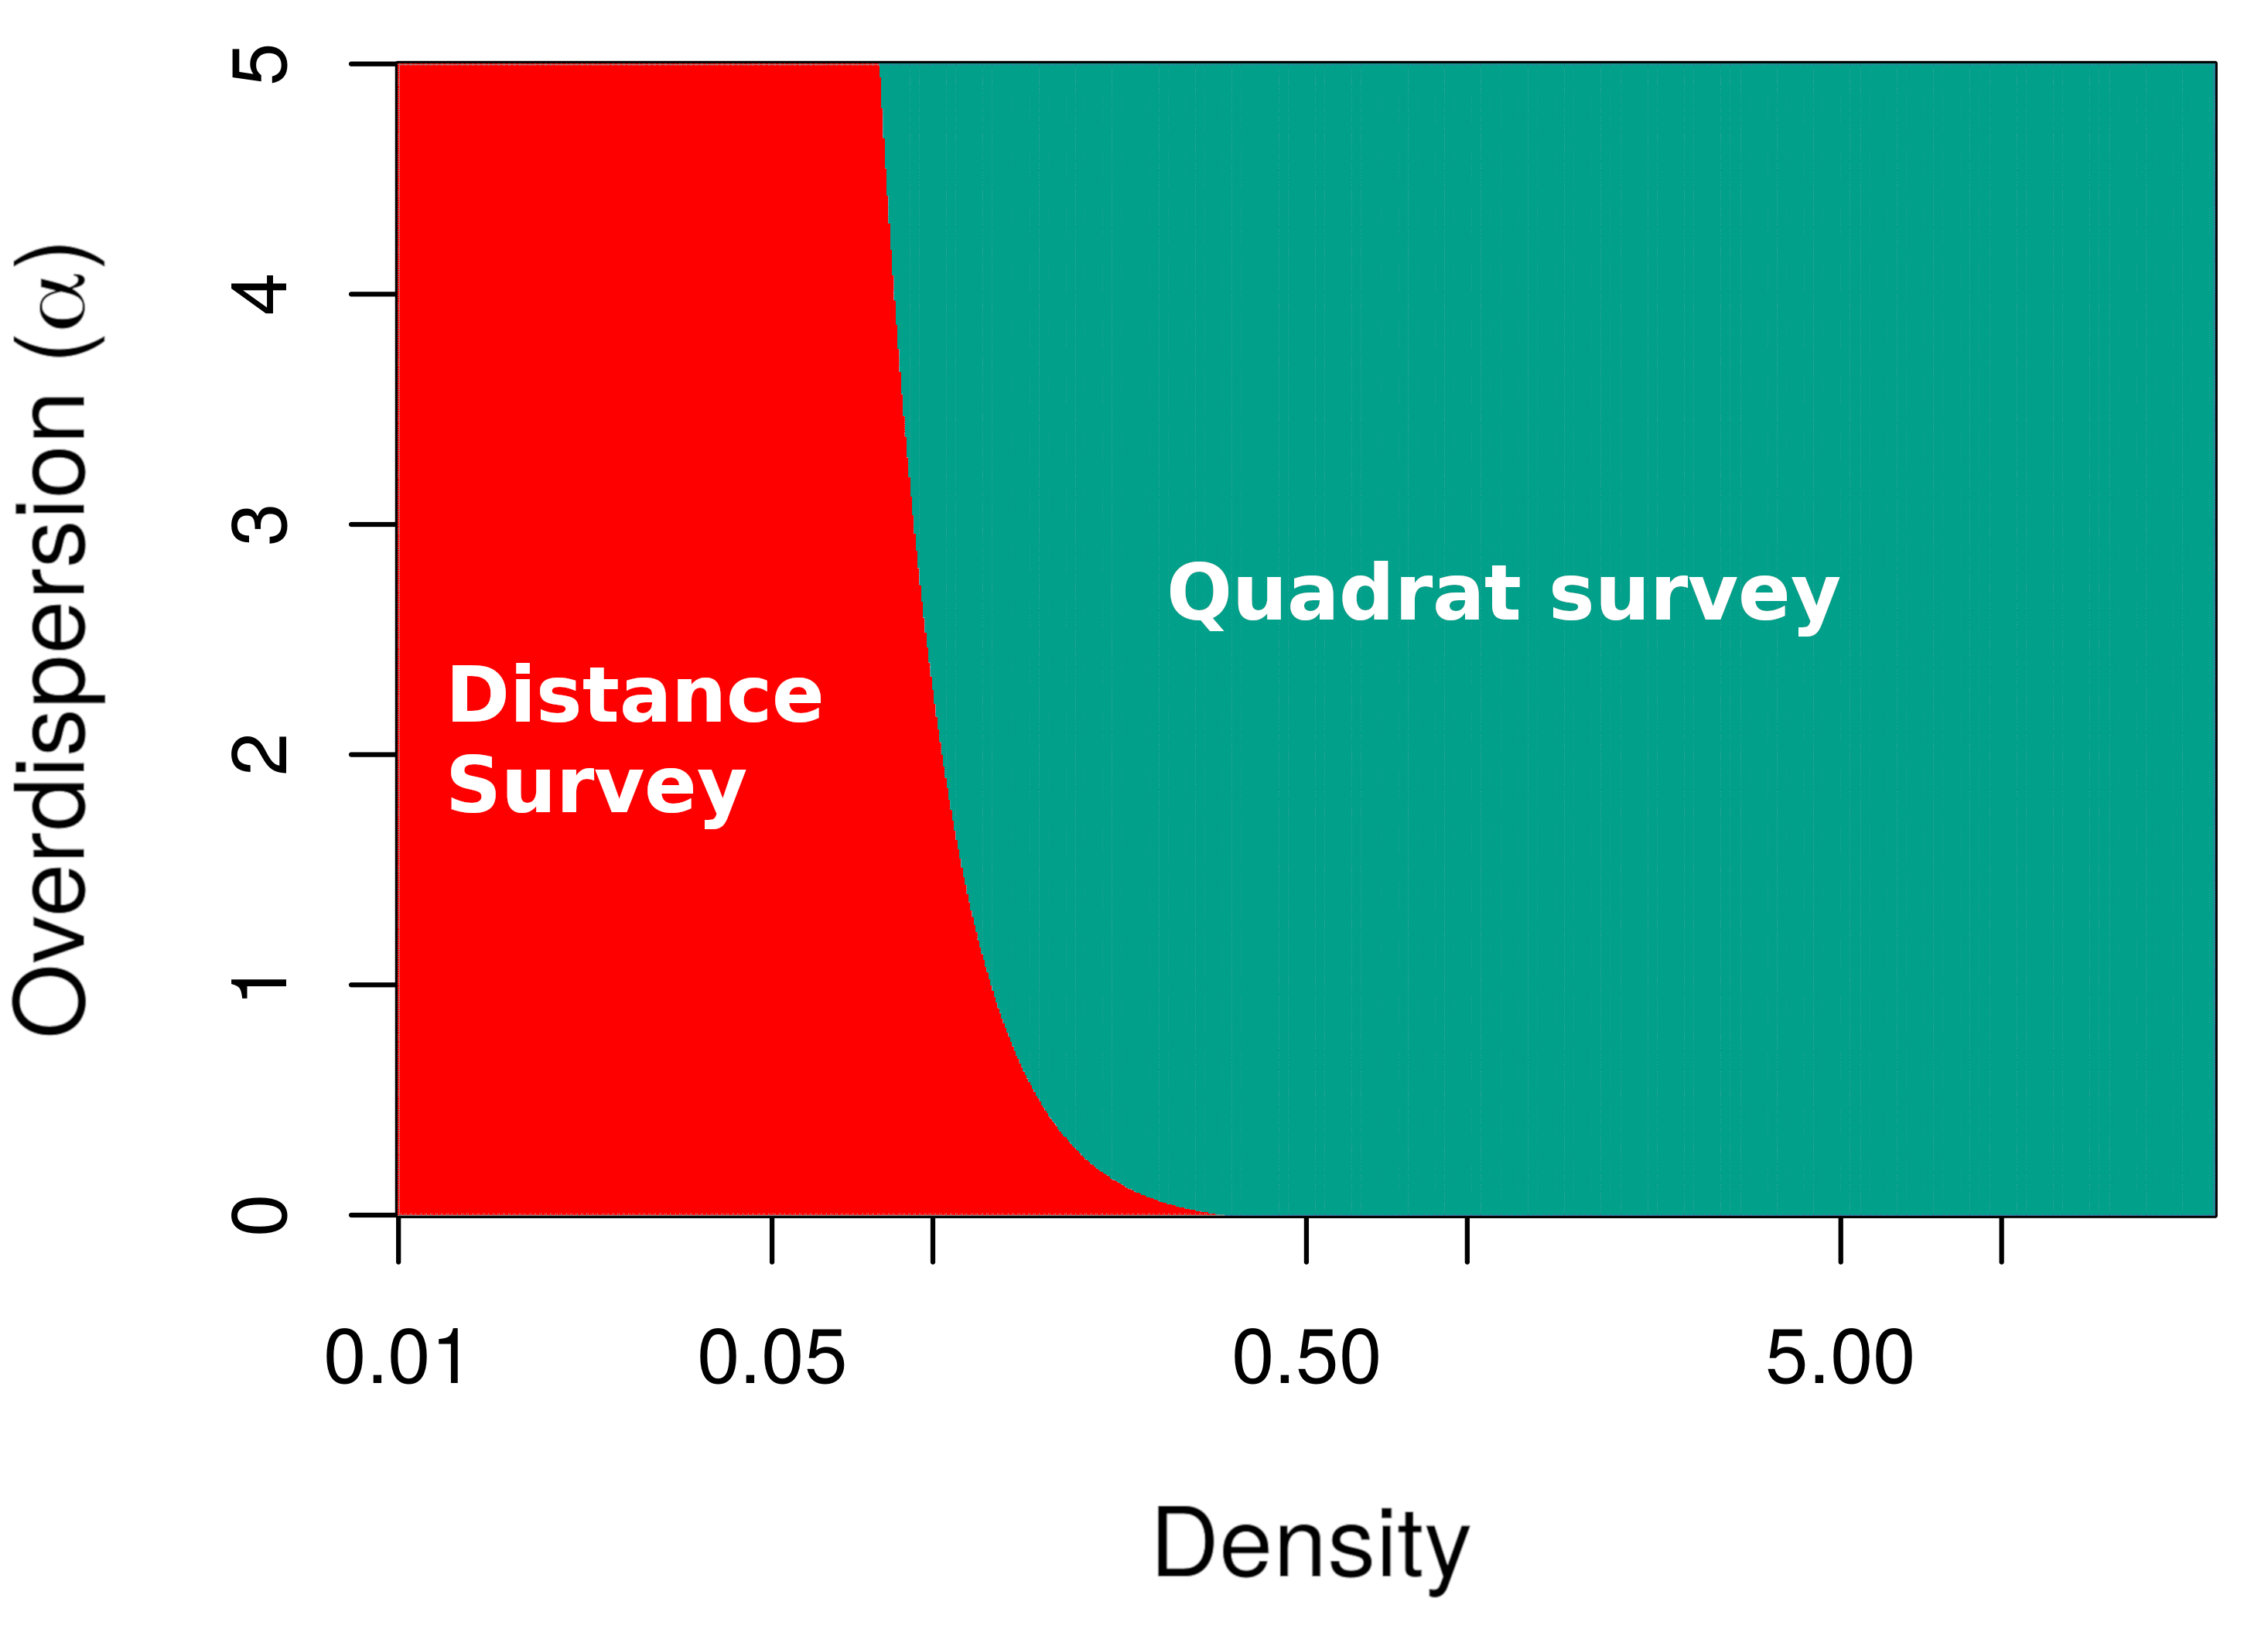
\includegraphics[width=0.65\linewidth]{../Figures/OptStrategy2} \end{center}

Predicts optimum changes at a \textbf{lower} density than we observed
empirically!

\end{block}

\begin{block}{Acknowledgements}

John Fieberg

Michael McCartney

Naomi Blinick

Leslie Schroeder

Sarah Baker

Aislyn Keyes

Austin Hilding

\href{mailto:jakeferg@hawaii.edu}{\nolinkurl{jakeferg@hawaii.edu}},
Snyder 414D

\end{block}

\begin{block}{Quadrat sampling error}

\begin{center}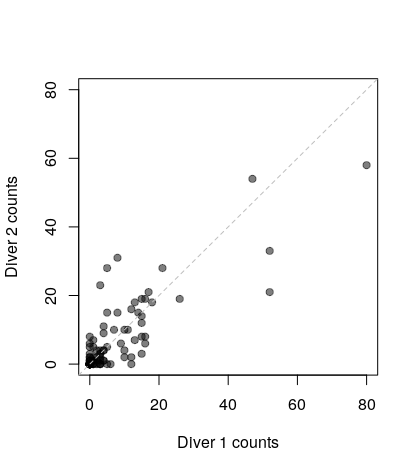
\includegraphics[width=0.5\linewidth]{../Figures/DiverCountComparison} \end{center}

\end{block}

\end{frame}

\end{document}
